\documentclass[12pt,reqno]{article}
% move all package loads to boilerplate file if poss
\usepackage[margin=1in]{geometry}
% \usepackage{fullpage}
% \usepackage[foot]{amsaddr}
\usepackage[utf8]{inputenc}
\usepackage[english]{babel}
\usepackage{braket}
\usepackage{mathtools}
\usepackage{caption}
% \usepackage{mathrsfs}
\usepackage{latexsym}
\usepackage{epsfig}

\usepackage{etoolbox}
\AtBeginEnvironment{quote}{\singlespacing\small}

\usepackage{lineno}


\usepackage{xcolor}
\usepackage{hyperref}
\usepackage{url}
\usepackage{setspace}
%\usepackage{breakurl}

\usepackage{url}
\makeatletter
\g@addto@macro{\UrlBreaks}{\UrlOrds}
\makeatother
\usepackage{xcolor}
\usepackage{float}
\usepackage{graphicx}

\oddsidemargin 0.25cm
\usepackage{morefloats}
\usepackage{tikz}
\usepackage{placeins}
\usepackage{cases}
\usepackage{footmisc}
\usepackage{dsfont}

\usepackage{booktabs}
\usepackage{amssymb}
\usepackage{amsmath}
\usepackage{adjustbox}
\usepackage{amsthm}
\usepackage{threeparttable}
\usepackage{epsfig}
\usepackage{graphicx}
\usepackage{caption}
\usepackage{subcaption}
\usepackage{lscape}
% \usepackage{scrwfile}
\usepackage{setspace}
\usepackage{multirow}
\usepackage{newclude}

\usepackage{todonotes}


\usepackage{lscape}
\newcommand{\bland}{\begin{landscape}}
\newcommand{\eland}{\end{landscape}}


\newcommand{\bburl}[1]{\textcolor{blue}{\url{#1}}}

\definecolor{maroon}{rgb}{0.5, 0.0, 0.0}

\hypersetup{breaklinks=true,
            bookmarks=true,
            pdfauthor={Apoorva Lal},
             pdfkeywords = {},
            colorlinks=true,
            citecolor=maroon,
            urlcolor=blue,
            linkcolor=blue,
            pdfborder={0 0 0}}
\urlstyle{same}  % don't use monospace font for urls

\makeatletter
\def\maxwidth{\ifdim\Gin@nat@width>\linewidth\linewidth\else\Gin@nat@width\fi}
\def\maxheight{\ifdim\Gin@nat@height>\textheight\textheight\else\Gin@nat@height\fi}
\makeatother
% Scale images if necessary, so that they will not overflow the page
% margins by default, and it is still possible to overwrite the defaults
% using explicit options in \includegraphics[width, height, ...]{}
\setkeys{Gin}{width=\maxwidth,height=\maxheight,keepaspectratio}

% \usepackage{tikz}
% \usepackage{tkz-tab}
% \usepackage{tkz-graph}
\usetikzlibrary{shapes.geometric,positioning}
\newcommand{\blue}[1]{\textcolor{blue}{(\bf{#1})}}
\newcommand{\emaillink}[1]{\textcolor{blue}{\href{mailto:#1}{#1}}}
\newcommand{\burl}[1]{\textcolor{blue}{\url{#1}}}
\newcommand{\fix}[1]{\textcolor{red}{\textbf{ (#1)\normalsize}}}
\newcommand{\fixed}[1]{\textcolor{green}{~\\ \textbf{#1\normalsize}}\\}
\newcommand{\ind}{\otimes}
\newcommand{\witi}{\widetilde}
\newcommand{\ch}{{\bf 1}}
\newcommand{\dt}[1]{\witi{\witi #1}}
\newcommand{\ol}[1]{\overline{#1}}
\newcommand{\lr}[1]{\left\lfloor#1\right\rfloor}
\newcommand{\eqd}{\overset{\footnotesize{d}}{=}}
\newcommand{\calf}{{\mathcal F}}

\renewcommand{\theequation}{\thesection.\arabic{equation}}
\numberwithin{equation}{section}


\usepackage{amsmath,amsfonts,amsthm,amssymb,amscd,bbm}

% command shorthand
\newcommand{\eg}{e.g., \xspace}
\newcommand{\ie}{i.e.,\xspace}
\newcommand{\etc}{etc.\@\xspace}
\newcommand{\iid}{\emph{i.i.d.}\ }
\newcommand{\etal}{et.\ al.\ }
\newcommand{\D}{\displaystyle}
\newcommand{\ba}{\begin{array}}
\newcommand{\ea}{\end{array}}
\newcommand{\be}{\begin{enumerate}}
\newcommand{\ee}{\end{enumerate}}
\newcommand{\bi}{\begin{itemize}}
\newcommand{\ei}{\end{itemize}}
\newcommand{\bs}{\begin{align}\begin{split}\nonumber}
\newcommand{\bsnumber}{\begin{align}\begin{split}}
\newcommand{\es}{\end{split}\end{align}}
\newcommand{\fns}{\singlespace\footnotesize}

% math shorthand
% vertical equal prefix
\newcommand{\verteq}{\rotatebox{90}{$\,=$}}
% vertical equal to
\newcommand{\equalto}[2]{\underset{\scriptstyle\overset{\mkern4mu\verteq}{#2}}{#1}}
% nullspace
\newcommand{\nulls}{\mathrm{null}}
% range
\newcommand{\range}{\mathrm{range}}
% maximise
\newcommand{\maximise}{\operatornamewithlimits{max}}
% minimise
\newcommand{\minimise}{\operatornamewithlimits{min}}
% maximiser
\newcommand{\argmax}{\operatornamewithlimits{arg\,max}}

% such that (inside math mode)
\newcommand{\suchthat}{\text{ s.t. }}

% indicator function
\newcommand*\Indic[1]{\mathbbm{1}_{#1}}

% big parentheses
\newcommand*\Bigpar[1]{\left( #1 \right )}

% convergence in probability sideways
\def\inprobLOW{\rightarrow_p}
% convergence in probability
\def\inprobHIGH{\,{\buildrel p \over \rightarrow}\,}
% convergence in probability 2
\def\inprob{\,{\inprobHIGH}\,}
% convergence in distribution
\def\indist{\,{\buildrel d \over \rightarrow}\,}

% equality in distribution
\def\eqdist{\,{\buildrel d \over = }\,}

% independence (bench)
\newcommand\indep{\protect\mathpalette{\protect\independenT}{\perp}}
\def\independenT#1#2{\mathrel{\rlap{$#1#2$}\mkern5mu{#1#2}}}

% ellipsis
\newcommand{\tto}{,\ldots,}

% blackboard F
\def\Function{\mathbb{F}}

% Lagrangian
\def\Lagr{\mathcal{L}}

% n-dimensional Real
\def\Realn{\mathbb{R}^n}

% P_n
\def\Probn{\mathbb{P}_n}

\def\rel{\,{\buildrel R \over \sim}\,}
% generic m x n matrix
\newcommand{\gmatrix}[1]{\begin{pmatrix} {#1}_{11} & \cdots &{#1}_{1n} \\ \vdots & \ddots & \vdots \\ {#1}_{m1} & \cdots &{#1}_{mn} \end{pmatrix}}

% Likelihood
\newcommand{\Likl}{\mathcal{L}}

% inner product
\newcommand{\iprod}[2]{\left\langle {#1} , {#2} \right\rangle}
% vector norm
\newcommand{\norm}[1]{\left\Vert {#1} \right\Vert}
% absolute value
\newcommand{\abs}[1]{\left\vert {#1} \right\vert}
% linalg misc
\renewcommand{\det}{\mathrm{det}}
\newcommand{\rank}{\mathrm{rank}}
\newcommand{\spn}{\mathrm{span}}
\newcommand{\row}{\mathrm{Row}}
\newcommand{\col}{\mathrm{Col}}
\renewcommand{\dim}{\mathrm{dim}}
% weakly prefer
\newcommand{\prefeq}{\succeq}
% strictly prefer
\newcommand{\pref}{\succ}
% sequence
\newcommand{\seq}[1]{\{{#1}_n \}_{n=1}^\infty }
% single arrow
\renewcommand{\to}{{\rightarrow}}
% double arrow
\newcommand{\corres}{\overrightarrow{\rightarrow}}
% evaluate definite integral
\newcommand*\Eval[3]{\left.#1\right\rvert_{#2}^{#3}}
% expectation
\newcommand{\Exp}[1]{\mathbb{E}\left(#1\right)}
% expectation at time
\newcommand{\Expt}[2]{\mathbb{E}_{#1}\left(#2\right)}
% variance
\newcommand{\Var}[1]{\mathbb{V}\left(#1\right)}
% Probability
\newcommand{\Prob}[1]{\mathbb{Pr}\left(#1\right)}
\newcommand{\F}{\mathscr{F}}
\newcommand{\f}{\widehat{\eta}}
%Blackboard Letters
\newcommand{\R}{\ensuremath{\mathbb{R}}}
\newcommand{\Z}{\ensuremath{\mathbb{Z}}}
\newcommand{\Q}{\mathbb{Q}}
\newcommand{\N}{\mathbb{N}}
\newcommand{\W}{\mathbb{W}}
\newcommand{\Qoft}{\mathbb{Q}(t)}  %use in linux

\newcommand\frakfamily{\usefont{U}{yfrak}{m}{n}}
\DeclareTextFontCommand{\textfrak}{\frakfamily}

% Fractions
\newcommand{\fof}{\frac{1}{4}}  %oneforth
\newcommand{\foh}{\frac{1}{2}}  %onehalf
\newcommand{\fot}{\frac{1}{3}}  %onethird
\newcommand{\fop}{\frac{1}{\pi}}    %1/pi
\newcommand{\ftp}{\frac{2}{\pi}}    %2/pi
\newcommand{\fotp}{\frac{1}{2 \pi}} %1/2pi
\newcommand{\fotpi}{\frac{1}{2 \pi i}}
\newcommand{\cm}{c_{\text{{\rm mean}}}}
\newcommand{\cv}{c_{\text{{\rm variance}}}}


% math shorthand
% vertical equal prefix

% minimiser
\newcommand{\argmin}{\operatornamewithlimits{arg\,min}}
% convergence in probability sideways
\def\inprobLOW{\rightarrow_p}
% convergence in probability
\def\inprobHIGH{\,{\buildrel p \over \rightarrow}\,}
% convergence in probability 2
\def\inprob{\,{\inprobHIGH}\,}
% convergence in distribution
\def\indist{\,{\buildrel d \over \rightarrow}\,}

% such that
\def\ST{\text{ s.t. }}

% if
\def\IF{\text{ if }}


% blackboard F
\def\Function{\mathbb{F}}

% Natural
\def\Nat{\mathbb{N}}
% Integers
\def\Int{\mathbb{Z}}
% Reals
\def\Real{\mathbb{R}}
% Rationals
\def\Rat{\mathbb{Q}}
% Complex
\def\Cplx{\mathbb{C}}

\newcommand{\reals}{\mathbb{R}} % Real number symbol
\newcommand{\integers}{\mathbb{Z}} % Integer symbol
\newcommand{\rationals}{\mathbb{Q}} % Rational numbers
\newcommand{\naturals}{\mathbb{N}} % Natural numbers

% n-dimensional Real
\def\Realn{\mathbb{R}^n}
% expectation_n
\def\Expn{\mathbb{E}_n}
% P_n
\def\Probn{\mathbb{P}_n}

\def\rel{\,{\buildrel R \over \sim}\,}



\renewcommand{\det}{\mathrm{det}}
\renewcommand{\dim}{\mathrm{dim}}
% single arrow
\renewcommand{\to}{{\rightarrow}}

\newcommand{\mc}[1]{\mathcal{#1}}
\def\mbf#1{\mathbf{#1}}
\def\mrm#1{\mathrm{#1}}
\def\mbi#1{\boldsymbol{#1}} % Bold and italic (math bold italic)
\def\v#1{\mbi{#1}} % Vector notation

\newcommand{\lone}[1]{\norm{#1}_1} % l1 norm
\newcommand{\ltwo}[1]{\norm{#1}_2} % l2 norm
\newcommand{\linf}[1]{\norm{#1}_\infty} % l-infinity norm
\newcommand{\dnorm}[1]{\norm{#1}_*} % Dual norm
\newcommand{\lfro}[1]{\left\|{#1}\right\|_{\rm Fr}} % Frobenius norm
\newcommand{\matrixnorm}[1]{\left|\!\left|\!\left|{#1}
  \right|\!\right|\!\right|} % Matrix norm with three bars
\newcommand{\matrixnorms}[1]{|\!|\!|{#1}|\!|\!|} % Small matrix norm
\newcommand{\opnorm}[1]{\matrixnorm{#1}_{\rm op}}
\newcommand{\opnorms}[1]{\matrixnorms{#1}_{\rm op}}
\newcommand{\normbigg}[1]{\bigg\|{#1}\bigg\|} % A norm with 1 argument and bigg
                                              % brackets.
\newcommand{\lonebigg}[1]{\normbigg{#1}_1} % l1 norm
\newcommand{\ltwobigg}[1]{\normbigg{#1}_2} % l2 norm
\newcommand{\linfbigg}[1]{\normbigg{#1}_\infty} % l-infinity norm
\newcommand{\norms}[1]{\|{#1}\|} % A norm with 1 argument and normal (small)
                                 % brackets.
\newcommand{\lones}[1]{\norms{#1}_1} % l1 norm with small brackets
\newcommand{\ltwos}[1]{\norms{#1}_2} % l2 norm with small brackets
\newcommand{\linfs}[1]{\norms{#1}_\infty} % l-infinity norm with small brackets

\newcommand{\hinge}[1]{\left[{#1}\right]_+}

\newcommand{\defeq}{:=}
\newcommand{\eqdef}{=:}
\newcommand{\what}[1]{\widehat{#1}} % Wide hat
\newcommand{\wt}[1]{\widetilde{#1}} % Wide tilde
\newcommand{\wb}[1]{\overline{#1}} % Wide bar

\newcommand{\half}{\frac{1}{2}}

\newcommand{\<}{\left\langle} % Angle brackets
\renewcommand{\>}{\right\rangle} % End angle brackets

\renewcommand{\iff}{\Leftrightarrow}
\renewcommand{\choose}[2]{\binom{#1}{#2}}  % Choose
\newcommand{\chooses}[2]{{}_{#1}C_{#2}}  % Small choose

%%%% Probability symbols and associated distances %%%%

\newcommand{\E}{\mathbb{E}} % Expectation symbol
\renewcommand{\P}{\mathbb{P}} % Probability symbol
\newcommand{\var}{{\rm Var}} % Variance
\newcommand{\cov}{\mathop{\rm Cov}} % Covariance
\newcommand{\simiid}{\stackrel{\rm iid}{\sim}}
\newcommand{\openleft}[2]{\left({#1},{#2}\right]} % Interval open on left
\newcommand{\openright}[2]{\left[{#1},{#2}\right)} % Interval open on right

\newcommand{\indic}[1]{\mbf{1}\left\{#1\right\}} % Indicator function

% Distances between probability measures
\newcommand{\tvnorm}[1]{\norm{#1}_{\rm TV}} % Total variation
\newcommand{\tvnorms}[1]{\norms{#1}_{\rm TV}}
\newcommand{\dkl}[2]{D_{\rm kl}\left({#1} |\!| {#2}\right)} % KL divergence
\newcommand{\dkls}[2]{D_{\rm kl}({#1} |\!| {#2})}  % Small KL-divergence
\newcommand{\dchi}[2]{D_{\chi^2}\left({#1} |\!| {#2}\right)}  % chi^2-divergence
\newcommand{\fdiv}[2]{D_f\left({#1} |\!| {#2}\right)} % f divergence
\newcommand{\kl}[2]{D_{\rm kl}\left({#1} |\!| {#2} \right)}
\newcommand{\dhel}{d_{\rm hel}}  % Hellinger distance
\newcommand{\helaff}{A_{\rm hel}}  % Hellinger affinity

% Convergence of random variables
\newcommand{\cd}{\stackrel{d}{\rightarrow}}
\newcommand{\cas}{\stackrel{a.s.}{\rightarrow}}
\newcommand{\cp}{\stackrel{p}{\rightarrow}}

\newcommand{\normal}{\mathsf{N}}  % Normal distribution
\newcommand{\uniform}{\mathsf{Uni}}  % Uniform distribution

% Simple floor/ceiling stuff
\newcommand{\floor}[1]{\left\lfloor{#1} \right\rfloor}
\newcommand{\ceil}[1]{\left\lceil{#1} \right\rceil}

\providecommand{\argmax}{\mathop{\rm argmax}} % Defining math symbols
\providecommand{\argmin}{\mathop{\rm argmin}}
\providecommand{\dom}{\mathop{\rm dom}}
\providecommand{\diag}{\mathop{\rm diag}}
\providecommand{\tr}{\mathop{\rm tr}}
\providecommand{\abs}{\mathop{\rm abs}}
\providecommand{\card}{\mathop{\rm card}}
\providecommand{\sign}{\mathop{\rm sign}}
\providecommand{\cl}{\mathop{\rm cl}}
\providecommand{\interior}{\mathop{\rm int}}
\providecommand{\conv}{\mathop{\rm Conv}}
\providecommand{\relint}{\mathop{\rm relint}}
\providecommand{\vol}{\mathop{\rm Vol}}
\providecommand{\supp}{\mathop{\rm supp}}

\providecommand{\minimize}{\mathop{\rm minimize}}
\providecommand{\maximize}{\mathop{\rm maximize}}
\providecommand{\subjectto}{\mathop{\rm subject\;to}}

% Proof environments
% The Theorems are numbered consecutively
% Lemmas are numbered by section, and observations, claims, facts, and
% assumptions take their numbering. Propositions and definitions have their
% own numbering by section.

\theoremstyle{plain}
\newtheorem{thm}{Theorem}[section]
\newtheorem{assumption}{Assumption}
\newtheorem{cla}[thm]{Claim}
\newtheorem{conjecture}[thm]{Conjecture}
\newtheorem{conj}[thm]{Conjecture}
\newtheorem{cor}[thm]{Corollary}
\newtheorem{defi}[thm]{Definition}
\newtheorem{egg}[thm]{Example}
\newtheorem{exe}[thm]{Exercise}
\newtheorem{hypothesis}[thm]{Hypothesis}
\newtheorem{lem}[thm]{Lemma}
\newtheorem{prob}[thm]{Problem}
\newtheorem{proj}[thm]{Research Project}
\newtheorem{proposition}[thm]{Proposition}
\newtheorem{propn}[thm]{Proposition}
\newtheorem{prop}[thm]{Proposition}
\newtheorem{que}[thm]{Question}
\newtheorem{rek}[thm]{Remark}
\newtheorem{rem}[thm]{Remark}
\newtheorem{X}{X}[section]


\renewenvironment{proof}{\noindent{\bf Proof}\hspace*{1em}}{\qed\bigskip\\}
\newenvironment{proof-sketch}{\noindent{\bf Sketch of Proof}
  \hspace*{1em}}{\qed\bigskip\\}
\newenvironment{proof-idea}{\noindent{\bf Proof Idea}
  \hspace*{1em}}{\qed\bigskip\\}
\newenvironment{proof-of-lemma}[1][{}]{\noindent{\bf Proof of Lemma {#1}}
  \hspace*{1em}}{\qed\bigskip\\}
\newenvironment{proof-of-proposition}[1][{}]{\noindent{\bf
    Proof of Proposition {#1}}
  \hspace*{1em}}{\qed\bigskip\\}
\newenvironment{proof-of-theorem}[1][{}]{\noindent{\bf Proof of Theorem {#1}}
  \hspace*{1em}}{\qed\bigskip\\}
\newenvironment{inner-proof}{\noindent{\bf Proof}\hspace{1em}}{
  $\bigtriangledown$\medskip\\}
%% \newenvironment{proof-of-lemma}[1][{}]{\noindent{\bf Proof of Lemma {#1}}
%%   \hspace*{1em}\renewcommand{\qedsymbol}{$\bigtriangledown$}}{\qed\bigskip\\}
\newenvironment{proof-attempt}{\noindent{\bf Proof Attempt}
  \hspace*{1em}}{\qed\bigskip\\}
\newenvironment{proofof}[1]{\noindent{\bf Proof} of {#1}:
  \hspace*{1em}}{\qed\bigskip\\}
\newenvironment{remark}{\noindent{\bf Remark}
  \hspace*{1em}}{\bigskip}


%



\renewcommand \thepart{}
\newcommand{\Ubr}[2]{\underbrace{#1}_{\text{#2}}}
\newcommand{\Obr}[2]{ \overbrace{#1}^{\text{#2}}}

% bibliography
\usepackage[
backend=biber,
style=authoryear,
citestyle=authoryear,
uniquename=false
]{biblatex}
\addbibresource{biblio.bib}

\renewbibmacro{in:}{}
\doublespacing
\setcounter{secnumdepth}{5}

\renewcommand{\footnotelayout}{\doublespacing \normalsize}
\setlength{\footnotesep}{0.9\baselineskip}

\newcommand{\figinc}[1]{\includegraphics[width=0.8\textwidth,height=0.8\textheight,keepaspectratio]{#1}}
\newcommand{\citep}[1]{\parencite{#1}}
\usepackage{minitoc}

\usepackage{unicode-math}
% \usepackage{floatrow}

\defaultfontfeatures{Ligatures=TeX,Scale=MatchLowercase}

\usepackage[T1]{fontenc}
\usepackage[utf8]{inputenc}
\setmainfont{XCharter}



% For word count:
% https://www.overleaf.com/learn/how-to/Is_there_a_way_to_run_a_word_count_that_doesn't_include_LaTeX_commands%3F?fbclid=IwAR0sjOa389OLM8ITZ6JU5raF_Med5kl7Qxl6otJLfhDqABVYM5qQaKl_s5A#Include_references_in_the_word_count


%%%%%%%%%%%%%%%%%%%%%%%%%%%%%%%%%%%%%%%%%%%%%%%%%%%%%%%%%%%%%%%%%%%%%%

\title{\textbf{Representation and Forest Conservation: \\ Evidence from India's Scheduled Areas}}

% \author{Saad Gulzar \\ Stanford \and Apoorva Lal \\
% Stanford  \and Benjamin Pasquale \\
% Independent Researcher\thanks{Gulzar is Assistant Professor, Stanford University (gulzar@stanford.edu). Lal is PhD candidate, Stanford University (apoorval@stanford.edu). Pasquale is an Independent Researcher (bjpasquale@gmail.com). We thank Rikhil Bhavnani, Mark Buntaine, Saumitra Jha, Teevrat Garg,  Alexandra Hartman, Steve Haber, Paul Novosad, Jonathan Rodden, Daniel Thompson, Gilles Verniers, and participants at the pre-APSA mini-conference on South Asia 2019, Asoka University, CEGA Evidence to Action Summit 2020, Pacific Conference for Development Economics 2020, Stanford Democracy Policy Lab, UCL, and Pia Raffler's replication class at Harvard, including Sachet Bangya, Byron Cohen, Chengyu Fu, and Kartik Srivastava for their valuable comments and suggestions. Surbhi Ghai provided excellent research assistance.}}


\date{\smallskip \today \\ Word count: 11979}


\begin{document}
\doparttoc % Tell to minitoc to generate a toc for the parts
\faketableofcontents % Run a fake tableofcontents command for the partocs

\thispagestyle{empty}
\maketitle

\begin{abstract} \singlespacing

Can representative institutions improve environmental conservation? We study the impact of a 1996 law that created local government with electoral quotas for Scheduled Tribes, a historically marginalized and impoverished community of 100 million in India. Using difference-in-differences designs paired with remote sensing data on deforestation, we find that formal representation reduces the rate of deforestation by thirty percent. These effects are larger in villages close to mines, where representation likely lowered commercial extraction. Combining these findings with research that the same institutions improved economic outcomes, our results challenge the commonly held assumption that there must be a trade-off between development and protecting the environment. While conservation policy tends to comprise environmentally-focused institutions, we suggest more attention be given to umbrella institutions, such as political representation, which can address conservation and development in tandem.

\end{abstract}



% \listoftodos

\newpage

\thepart{}
%%%%%%%%%%%%%%%%%%%%%%%%%%%%%%%%%%%%%%%%%%%%%%%%%%%%%%%%%%%%%
\setcounter{page}{1}
\section{Introduction} % (fold)
\label{sec:introduction}

% \linenumbers
% \modulolinenumbers[5]

% #### ##    ## ######## ########   #######
%  ##  ###   ##    ##    ##     ## ##     ##
%  ##  ####  ##    ##    ##     ## ##     ##
%  ##  ## ## ##    ##    ########  ##     ##
%  ##  ##  ####    ##    ##   ##   ##     ##
%  ##  ##   ###    ##    ##    ##  ##     ##
% #### ##    ##    ##    ##     ##  #######


%% BIG PICTURE - WHAT ARE WE TALKING ABOUT? WHY DO WE CARE? 

The Earth's future climate likely depends, to a large extent, on our ability to preserve forest ecosystems. Deforestation both exacerbates climate change and decreases biodiversity \parencite{bonan2008forests} -- accounting for 12-20\% of annual greenhouse gas emissions, and eclipses all transportation related emissions \parencite{solomon2007ipcc}. Forest areas often lie on the fringe of state influence and require balancing of immediate concerns over economic livelihoods of marginalized populations living in those areas with the pressing need to guarantee renewable resources for future generations. 

Designing policies that are sensitive to these dual considerations is particularly pressing in developing countries --  in just India, Indonesia, Nepal, the Philippines, Sri Lanka, and Thailand about 447 million poor and marginalized individuals depend on forests \parencite{lynch1995balancing}. In addition, while indigenous populations only comprise five percent of the global population, they manage a quarter of Earth's land surface and support 80 percent of its biodiversity \parencite{garnett2018spatial}. Recent research tends to examine policies that target conservation {\it or} development. For instance, work on conservation has tested the efficacy of various environmental monitoring regimes that prevent over exploitation \parencite{anderson2019non,buntaine2020combining,metaketaiii,Christinsen2020}, institutions that assign property rights \parencite{buntaine2015titling,baragwanath2020collective} and also those that give subsidies to prevent over-logging \parencite{samii2014effects,jayachandran2017cash}. 

%The risks of deforestation present an unresolved global and local problem: have been widely discussed \parencite{stern2006economics}, they 

%the challenge of keeping logging at or below a sustainable level, while maintaining those resources as important sources of livelihood for those living in close proximity. 

%This trade off is especially pronounced in developing countries, where deforestation has grown rapidly and conservation efforts are limited by weak state capacity. Moreover, 


%%% WE STUDY POL REP / QUOTAS

We examine another type of institution, one explicitly designed to take an \emph{umbrella} approach to the dual policy problems of improving development outcomes for marginalized and poor communities living in proximity to natural resources, and conserving those very resources. We study increasing political representation via formal elected bodies, under whose aegis lies both the protection and use of forest resources as well as the implementation of large-scale government programs.  


%%% THEORETICAL PUZZLE

Theoretically, it is unclear whether increasing representation for marginalized local communities will increase extraction or conservation of environmental resources. Examined classically, control by local communities could increase overuse by enabling local actors to displace central leadership, thereby exacerbating the tragedy of the commons \parencite{hardin1968tragedy}. More recent work suggests that environmental governance can actually be quite effective with local control \parencite{ostrom1990governing}, though evidence from a variety of contexts has been mixed. We suggest a key reason for this mixed evidence in the literature: control of resources is often not accompanied by an effective transfer of formal \emph{political power} to local communities. We argue that increased political representation for marginalized communities, who see preservation as congruent with their own long term well-being, will increase conservation. We model these ideas and derive observable implications for empirical testing.

% remains under-examined is an assessment of whether these institutions curb or exacerbate the overuse of renewable resources.

%Theoretically, the effects of decentralisation on resource use are  ambiguous. On the one hand, many environmental studies scholars show considerable enthusiasm in favour of decentralisation, citing its benefits as arising from the congruence between the unit affected by resource-use decisions and those making them. This position is concisely articulated by \textcite{Lemos2006-tq} argue that decentralisation may facilitate preservation through three channels: ``It can produce greater efficiencies because of competition among sub-national units; bring decision making closer to those affected by governance, thereby promoting higher participation and accountability; and it can help decision makers take advantage of more precise time- and place-specific knowledge about natural resources.'' On the other hand, increasing the number of `sellers' in a market through decentralisation could potentially exacerbate the `tragedy of the commons' problem: in a Cournot setup, an increase in the number of firms leads to lower prices of forest produce and increase quantity produced (that is, increase deforestation) \parencite{Burgess2012-hk}. The sign of the net effect, therefore, is theoretically ambiguous yet important for public policies that aim to improve conservation.

% Context and policy contribution
%, given its, (a) large rural population, a lot of which is dependent upon the forests, (b) a complex history of forest extraction, conservation and deforestation, and (c) a unique quota system that dramatically increased representation for the historically disadvantaged Scheduled Tribes, the individuals most affected by forest produce and deforestation. 



% CASE / CONTEXT

We examine the case of India, a critical context to study the effects of political representation on deforestation. Of India's total population, $66$\% live in rural areas, 275 million depend on the use of forest resources \parencite{RupeeFund}, and 100 million are associated with the Scheduled Tribe (ST) identity category, a category grouping those commonly understood to be the country's most economically vulnerable and politically excluded, who  are concentrated in heavily forested and geographically frontier areas. ST may be compared to the many indigenous communities around the world who rely on forest produce to meet their caloric intake, sell minor forest produce to earn a livelihood, and practice sustainable agriculture \parencite{kashwan2017democracy, zimmerman2001conservation}.

Shortly after Independence, The Parliament of India declared certain regions in the country as Scheduled Areas, a territorial category linked to the protection of a historically disadvantaged category of minority groups -- the Scheduled Tribes. From 2000, under the Panchayat Extension to Scheduled Areas (PESA) Act of 1996, India’s national parliament extended local government councils to Scheduled Areas and implemented an electoral quota that required all chairperson positions in three tiers of local government councils, as well as at least half the seats on each of those councils, be reserved for ST individuals. In other, non-Scheduled, areas of India, local government had already recently been implemented under the Constitution (73rd Amendment) Act of 1992 (known widely as the Panchayati Raj Act) but without the same political reservations for Scheduled Tribes. We study the impact of increased political representation for Scheduled Tribes on deforestation. 


%Centralized forest policy has historically favored extraction instead of conservation or development. Prior to Independence, the British enacted legislation to limit the rights of forest inhabitants and forest users, with the aim of extracting resources and retaining the exclusive use of forests. These policies were re-imagined yet continued and expanded upon after Independence from the British. 

%More recent debates in India center on how and whether to balance conservation efforts with the development of communities living on the fringes of forests. However, despite forest conservation movements and rebellions, meaningful legislative change was limited until the Panchayat Extension to Scheduled Areas of 1996, which dramatically increased the political representation of the Scheduled Tribes.

%Arguably none of the political quotas analyzed in the literature have been as significant (and as previously under-examined) as the Scheduled Areas quota targeting the Scheduled Tribes - a category accounting for over 100 million Indian citizens. In some form, political quotas have been adopted by more than 100 countries across the world. These institutions seek to empower historically marginalized communities in places where elite capture reduces the representativeness and efficacy of elected political bodies. While previous work has studied the development impacts of these institutions, and found mostly positive effects, including on the provision of public goods and government responsiveness more broadly (see for example \textcite{jensenius2017social,gulzar2019})\todo{add a more comprehensive list of cites here}, the extent to which these elected bodies ameliorate or exacerbate the overuse of common pool resources remains under-examined. Beyond institutions like quotas that align effect of the existence and composition of elected local governments on common pool resource utilization is under-examined and merits further study because of the role they play in coordinating and aggregating natural resource utilization preferences amongst the electorate and decisions pertaining to those resources.

%The other important set of policies was mandating increased political representation for an array of historically underrepresented and vulnerable identity groups since Independence from the British. 

%Rural forest dwellers have been impacted not only by government policy, but the rate of deforestation in India has also been exacerbated by population growth and industrialization. Forest cover has decreased from roughly 40\% in the 1850s to less than 20\% in the 1990s \parencite{lynch1995balancing}. 

% -- many of whom are forest-dependent, historically marginalized and vulnerable\todo{@ben this parenthetical can be removed after you write the above} -- 



%%% RESEARCH DESIGN 

Estimating the causal effects of political institutions on forest preservation efforts is difficult for several reasons. First, because political institutions are usually either implemented simultaneously over large administrative units (e.g. an entire country). Second, reforms may be selectively implemented, but done so for areas that are unrepresentative, or simply trending differently to, other parts of the country. Both of these create problems for the construction of a suitable counterfactual. The dramatic increase in representation for ST in already established Scheduled Areas, under PESA, presents a unique opportunity to study the impact of representation on deforestation. We leverage the state-level staggered adoption of elected, local government councils, as well as within-state variation in PESA areas, for two distinct difference-in-differences designs. This enables us to isolate the causal effect of the PESA local election with quotas on deforestation. 

In addition to the causal identification challenge, measuring systematic, local changes in deforestation over large areas and over long periods of time, has until recently been impossible for social scientists. While early work, such as sections of seminal books by \textcite{ostrom1990governing} and \textcite{ellickson1991order}, made use of detailed case-studies and fieldwork in small communities, political scientists have seldom used novel remote-sensing micro data that have only recently become available from satellites such as LANDSAT, Sentinel, and DMSP. We introduce the use of one such dataset and invite political scientists to make more use of large scale, high throughput datasets produced by environmental scientists and geographers. These data enable us to trace local changes in deforestation rates over the long run, from 2001 to 2017, at the arc second(30m $\times$ 30m) grid cell level, which is the finest resolution available for civilian scientific use. %This allows us to understand whether a given village in our sample experienced deforestation in a given year.


%% EMPIRICAL RESULTS

Our main finding is that broadening formal representation for Scheduled Tribes led to a {\it thirty percent} reduction in deforested area, a statistically and substantively meaningful decrease. Importantly, the effects are larger for areas that had more forest cover at the start of the study period. We show that our observed effects arise only after the introduction of PESA elections that mandate quotas for ST, suggesting the importance of electoral politics in changing deforestation outcomes. 

Next, we empirically examine a potential mechanism for the effect of representation on deforestation -- the relationship between mining and forest conservation. Industrialization in India, and mining in particular, have long been considered causes of environmental degradation, and a major impediment to conservation \parencite{roy2011walking, saha2011under, areendran2013land, downing2002avoiding}. A motivating factor for the Indian state's legislative efforts to protect forest resources was to support local communities against large and well-financed mining interests. First, we find that areas that are close to mines at the beginning of our sample window, prior to the implementation of PESA, were deforested at higher rates. Second, the introduction of PESA elections leads to a greater reduction in deforestation for PESA villages close to any mines, and is even higher for villages near multiple mines. We interpret these results as showing how increased representation may empower ST to limit mining in their areas, which is consistent with qualitative accounts of mining in India.

Finally, we unpack representation into its constituent parts - the presence of local government and mandated representation for ST. To do so, we examine the case of Jharkhand, which held its first local elections for \emph{both} Scheduled and non-Scheduled Areas in 2010, unlike the rest of India. As a result, the only difference between Scheduled and non-Scheduled Areas in Jharkhand after 2010 is the presence of the ST quota. We find particularly strong evidence for the effects of mandated representation on deforestation in Jharkhand.


%we analyze the case of Jharkhand, which held its first local elections, in the entire state, at the same time in 2010. We argue that if we find similarly large effects in Jharkhand, treatment effects are likely driven by mandated representation for ST rather than the arrival of local governments. Consistent with this, our evidence shows that mandated representation is a key element in addressing the historical absence of political voice for ST in rural India.

%While we have made the case for the importance of both, the case of Jharkhand allows some insight of the relative impact of quotas on deforestation. Due to legal battles regarding the independence of the state of Jharkhand in 2010 \footnote{Jharkhand separated from Bihar in 2000, alongside Chhattisgarh and Uttrakhand.}, Jharkhand held its first local elections for \emph{both} Scheduled and non-Scheduled Areas in 2010. For this reason, Jharkhand's first post-PESA election in 2010 introduced local elections effectively to the entire state, and quotas-only in Scheduled Areas. 

%In this way, formal political control over resources, by local communities, is perhaps a powerful tool for marginalized communities to preserve the renewable resources upon which their livelihoods depend.

%We also evaluate whether the election of ST leaders is sufficient for improvements in conservation, or whether electoral demands are necessary for conservation effectiveness. To do so, we decompose the effect of PESA introduction across the distribution of ST population share in our sample, and find that effects are largely similar across ST-plurality and ST-non-plurality villages, suggesting that it is the election of an ST leader that is the primary mechanism for change rather than an increased demand to stop deforestation following the implementation of PESA. 


%%% DISCUSSION / RETURNING TO CONSERVATION v DEVELOPMENT

Having found a clear relationship between local representation and conservation, we return to the question of whether increased conservation comes only with corresponding economic costs for historically marginalized communities. We combine this paper's findings with other research, that examines the same policies, but focuses instead on economic outcomes. Contrary to concerns that environmental protection must come at the cost of local development, \textcite{gulzar2019} find that the improvement in representation for Scheduled Tribes, in the same context, led to (1) large increases in the economic welfare for ST as measured by the performance of the world's largest workfare program, (2) improvement in local road connectivity, and (3) general improvements in the provision of public goods.%\footnote{See [citation omitted] for details.}

%%% CONTRIBUTIONS

This paper makes theoretical, empirical and policy contributions. Theoretically, we clarify competing predictions and results from a large literature that examines the efficacy of local political control on conservation. Our results highlight how one reason for mixed evidence on how local control affects natural resources use, may be because decentralization is frequently not accompanied by institutions that truly create space for marginalized voices.  

Empirically, we pair new remote-sensing, high-resolution data on deforestation with a longitudinal, quasi-experimental research design. This constitutes a major advance over related previous work in political science and environmental science: much of this literature has relied on either cross-sectional, or before-after comparisons, as ways of identifying the effects of policies on environmental outcomes, both of which struggle to credibly identify causal effects. By leveraging a unique policy and its roll out, we provide credible evidence of how improved political representation for marginalized communities reduced natural resource extraction. In doing so, we contribute to a small but emerging literature that pairs environmental data sets with modern research designs to study the effects of public policy on environmental outcomes \parencite{ferraro2020conditional, baragwanath2020collective,sanford2021democratization}.

From a policy perspective, the paper presents evidence that conservation and the social protection of marginalized populations need not be substitutes. Our evidence from rural India suggests that the two policy objectives may indeed be complementary. In this sense we advocate greater attention be paid to umbrella political institutions that includes in their design concerns of both development and conservation. Such institutions are distinct from others that focus exclusively on conservation or development, both of which are frequently studied in isolation.

%The remainder of the paper is organized as follows: section \ref{sec:conceptual_framework} places the research in relevant literature, section \ref{sec:context} provides further institutional details, section \ref{sec:data} describes the various data sources and the construction of our analysis sample, section \ref{sec:empirical_strategy} describes our empirical strategy, section \ref{sec:Results} reports our results and reports some extensions and robustness checks that we perform to validate our results. Section \ref{mechanisms} probes some mechanisms, and section \ref{sec:conclusion} concludes.% section introduction (end)

% ######## ##     ## ########  #######  ########  ##    ##
%    ##    ##     ## ##       ##     ## ##     ##  ##  ##
%    ##    ##     ## ##       ##     ## ##     ##   ####
%    ##    ######### ######   ##     ## ########     ##
%    ##    ##     ## ##       ##     ## ##   ##      ##
%    ##    ##     ## ##       ##     ## ##    ##     ##
%    ##    ##     ## ########  #######  ##     ##    ##

\section{Political Representation and Resource Preservation} % (fold)
\label{sec:conceptual_framework}

In this section we introduce a simple theoretical framework on how various institutional arrangements may affect the extraction of natural resources in our context. We review competing accounts, and mixed evidence, of how institutions exacerbate or attenuate environmental conservation. We suggest a new reason to explain why local institutions have often failed to improve resource conservation -- the absence of effective political representation. We return to our theoretical framework to formalize our prediction and conclude with observable implications. 





\subsection{The Tragedy of the Commons}\label{sub:toc_mod}

Common-pool resources have long suffered the `tragedy of the commons,' where individual decisions to extract result in aggregate overuse and resource depletion \parencite{hardin1968tragedy}. Centralized control over the utilization of a resource, as opposed to more local management by communities closest to the resource, is classically seen as a solution to this problem because local decision-makers fail to accurately account for their own overuse, leading to negative externalities and aggregate overuse. 

To illustrate this logic formally, consider $n$ villages with a common forest, and let $X = \sum_{i=1}^N x_i$ be the total number of trees felled by all villages.\footnote{We assume resource utilization decisions are made unilaterally within each village by village elites with no citizen input.} The value of each tree is $p$. The cost of logging is $c(X)$ (where $X$ is the \emph{aggregate} level of logging, which is how we embed externalities in this setup -- increased logging by $i$ increases costs for everyone), where $c'(X) > 0$ and $c''(X) > 0, c(0) = 0$. So, the cost of logging is increasing in total trees felled, at an increasing rate. Importantly, this cost is common across villages and therefore over-utilization by one village increases costs for all villages, capturing externalities and spillovers related from individual decisions.  The payoff to village $i$ is

\begin{equation}
 v(x_i) = [p - c(X)] x_i = \left(p -  c \left( \sum_{j=1}^n x_j\right)\right) x_i \label{eqn:vil_prob}
\end{equation}

The total payoff for all villages from logging $X$ trees is  $W(X) = [p - c(X)]X$. So, the socially optimal number of trees to fell is defined as the first order condition (FOC) with respect to the \emph{total} number of trees felled $X$ summing \ref{eqn:vil_prob} across villages, which is
\begin{equation}
 0 = \Ubr{p}{MSB} - \Ubr{[c'(X^{fb}) X^{fb} + c(X^{fb})]}{MSC} \label{eqn:soc_opt}
\end{equation}

This equates the marginal social benefit (MSB) of logging an additional tree $p$ with the marginal social cost (MSC). However, now consider the solution to an individual village's decision problem, \ref{eqn:vil_prob}, which is characterized by the FOC
\begin{equation}
0 = \Ubr{p}{MPB} - \Ubr{[c'(X) x_i^* + c(X)]}{MPC} \label{eqn:eqn_foc}
\end{equation}

\noindent which equates marginal \emph{private} benefit (MPB) to marginal \emph{private} cost (MPC). All villages choose optimally, which is the unique Nash equilibrium of the game. Summing this first-order condition over villages $i$ and dividing by $n$ gives us an equation in the total equilibrium logging $X^*$ when each village is logging independently,
\begin{equation}
0 = p - \left[ \frac{1}{n} c'(X^*) X^* + c(X^*) \right]
\label{eqn:ind_opt}
\end{equation}

Equilibrium utilization under the social optimum and independent decision-making are implicitly defined in \ref{eqn:soc_opt} and \ref{eqn:ind_opt}. While deriving an explicit expression requires fully specifying the cost function $c(\cdot)$, we can state the result that $X^* > X^{fb}$ without any functional form assumptions. In particular, the coefficient $1/n$ on $c'(X^*)X^*$ implies that $X^* >
X^{fb}$.

\begin{propn}[$X^* > X^{fb}$]\label{prop:trag_propn} Independent decision-making results in more logging than the socially optimal level.
Proof in appendix \ref{ssub:proof_to_proposition_prop:trag_propn}.
\end{propn}

In summary, equating marginal private benefit to marginal private cost (under the independent decision-making regime), results in overutilization and does not generate socially optimal outcomes that are externalities. This is the classic tragedy of the commons result.

\subsection{How Local Control May Improve Conservation}

While some recent research has found evidence for the tragedy of the commons \parencite{lopez1998tragedy}, in general, it remains unclear if centralized strategies for resource conservation are effective at curbing resources overuse. Evidence from 137 countries suggests that countries with less democratic institutions are more likely to restrict access to forests \parencite{kashwan2017inequality}, perhaps so that kickbacks may be obtained through access licenses. 

Elinor Ostrom proposed an alternative, where central control was problematic because ``the optimal equilibrium achieved by following the advice to centralized control... is based on assumptions concerning the accuracy of information, monitoring capabilities, sanctioning reliability, and zero costs of administration'' by the central authority \parencite[10]{ostrom1990governing}. Instead, Ostrom argued that environmental resources could be effectively governed by the local communities using them, rather than central government regulation or private companies. Consistent with this, recent research highlights problems with centralized control even in settings where state capacity is high, as in China \parencite{anderson2019non}.  

Scholars of environmental governance, such as \textcite{sethi1996evolution, dasgupta1995inquiry, agrawal1999enchantment,Dietz2003-bs,Lemos2006-tq}, have argued that local control of renewable resources can work through the internalization of social norms towards sustainable use. Yet the evidence to date has been mixed. Examining the effects of various institutional protections to local, indigenous communities, on deforestation outcomes, research has found positive, negative, and null effects.\footnote{For positive results see \textcite{baragwanath2020collective,nolte2013governance,nepstad2006inhibition,robinson2014does,bonilla2019protected,blackman2017titling,agrawal2014governing}; for negative results see \textcite{robinson2014does, benyishay2017indigenous, buntaine2015titling}; and for null effects see \textcite{Christinsen2020}.}

%\textcite[506]{agrawal2001collective} assert that ``the cases in which there has been most effective decentralization in property rights are also the ones in which forest conditions have improved.''
%\textcite{feeny1990tragedy}
%This wave of scholarship examined the impacts of decentralization policies that were increasingly adopted across the world since at least the 1990s.  %\textcite{agrawal1999enchantment} outline the importance of `institutions' at the community level to aid the management of renewable resources.

%Furthermore, as local communities now control more than 13 percent of the world's forests \parencite{oldekop2019reductions}, it is important that we examine how specific features of local institutions moderate their efficacy towards ameliorating free-riding problems \parencite{ostrom1990governing, agrawal1999enchantment, Berkes15188}. 

%This absence may explain mixed findings in the literature, particularly as it relates to elite capture \citep{bardhan2000capture}. Political institutions that elect leaders prefer resource conservation may therefore be particularly effective at reducing deforestation \parencite{aklin2018prisoners}. 

%Two features of our focus on political representation are distinct from previous research: (1) , and (2) we study an umbrella institution that, rather than solely focusing on conservation, addresses multiple dimensions of public policy. 

%We focus on bolstering representation by means of a quota making local government less susceptible to elite capture.

%The first distinction relates to the absence of real political power for marginalized communities. -- communities who have the most to gain through the preservation of natural resources

%Local community led institutions may improve local communication, increase trust, lower the cost of monitoring and increase rule compliance, all of which may attenuate over-extraction \parencite[1908]{Dietz2003-bs}.

\subsection{The Role of Representation}

These mixed findings may be driven by institutions that provide authority to local decision makers, but do not make adequate arrangements to truly boost the voice of marginalized communities in resource management. One way to dramatically increase the political voice of historically excluded and economically vulnerable populations is through electoral quotas. Quotas -- often referred to as {\it reservations} in the Indian context -- are present across more than 100 countries around the world, but their efficacy vis-a-vis deforestation has not been systematically examined. %\textcite[303]{Lemos2006-tq}  argue that local control may facilitate preservation through three channels: increasing local government unit competition, bringing decision-making closer to those who are directly affected, thereby increasing participation and accountability, and by empowering decision-makers who have knowledge of local and current conditions. 

Effective political representation, from hinterland communities who sit at the frontier of human settlement, may be particularly effective as state capacity is weak in these areas. Indeed, scholars argue that ``empowering pro-climate constituencies across countries'' holds great promise in solving problems related to climate change \parencite[6]{aklin2018prisoners}. Finally, a formal political institution, such as mandated representation through quotas, is likely to address and improve along many, if not all, dimensions that Ostrom identifies as design principles for robust common pool resource management \parencite[90]{ostrom1990governing}. % which we return in the Indian context, in the following section.

To incorporate ST representation into the model we introduced in \ref{sub:toc_mod}, we separate the cost function $c(X)$ into two parts: $c_G(X)$ is a global cost from depletion (which inherits the properties of $c(\cdot)$, and therefore is a function of \textit{aggregate utilization} $X$). $c_G(\sum_i x_i)$ is global in the same sense as before: by incorporating externalities. By contrast, $c_L(x_i)$ is now a local cost incurred from deforestation by leaders whose electorates have a particular aversion to resource depletion. This local component of the cost is a substantive modeling assumption driven by the case of ST in India. It also yields a natural assumption that $c_L'(\cdot) > c_G'(\cdot)$, that is, local costs from deforestation grow faster than global costs. 

We incorporate improved representation in a reduced-form way by defining $\alpha \in [0, 1]$ which denotes the degree to which local resource utilization decisions must align with local utilization preferences.\footnote{The parsimony of our current approach, which abstracts from an explicit electoral stage, is appropriate because our empirical focus is on representation of ST across space, relative to the intensive margin through an electoral model with policy competition in local preferences over extraction.} PESA villages have a strictly positive value $\alpha > 0$. The payoff for each village is now
\begin{equation}
 v(x_i) = \left[p- (1-\alpha) c_G(x)- \alpha c_L(x)\right] x_{i}
 \label{eqn:vil_prob2}
\end{equation}

\noindent This nests the fully independent decision-making setup we discussed in \ref{sub:toc_mod} as a special case where $\alpha = 0$.  The above objective function yields  the corresponding first-order condition with respect to $x_i$:
\begin{equation}
0 = p-\left[
    (1-\alpha)\Obr{
        \left\{c_G^{\prime}(X) x_{i}^{rep}+c_G(X) \right\}}{Global marginal cost} +
    \alpha
    \Obr{
        \left\{c_L^{\prime}(x_{i}^{rep}) x_{i}^{rep}+
        c_L(x_{i}^{rep})\right\}}{Local Marginal Cost}
    \right]
\end{equation}

This FOC collapses to \ref{eqn:ind_opt} when $\alpha = 0$, so that villages who do not weigh local costs at all, deforest at the same rate as in the case of fully independent decision-making. However, for villages that do consider local costs heavily (i.e. where $\alpha > 0$), the utilization decision yields a new optimum $x_i^{rep}$, equilibrium logging under greater local representation that places a positive weight on local costs.

\begin{propn}[$X^{rep} < X^{*}$]\label{prop:repr_propn} Independent decision-making with local representation results in less logging than under independent decision-making alone. 
Proof in appendix \ref{ssub:proof_to_proposition_prop:repr_propn}.
\end{propn}

Without further assumptions about $c_G$ and $c_L$, we are unable to rank $X^{fb} \lessgtr X^{rep}$, though substantively, it is unlikely that even independent decision-making attains the socially optimal level of utilization. However, for our purposes, it is sufficient that we have proved $X^{rep} < X^{*}$, which is the key empirical prediction we take from this formal framework, to the data. That is, we expect that effective local representation for communities who value forest resources should reduce deforestation rates, relative to institutional arrangements that provide local control without an effective formal representation apparatus for these communities. 

%This states that once local politicians are compelled to take local preferences into account in the process of resource utilization, the equilibrium level of resource utilization can be expected to be strictly lower relative to situations where no such costs are incurred.Furthermore, the pre-PESA equilibrium of decentralized decision making can hardly be characterized as first-best given the possibility of corruption with distant, concentrated bureaucratic power.



% section conceptual_framework (end)
%
%  ######  ######## ##     ## ########
% ##    ##    ##     ##   ##     ##
% ##          ##      ## ##      ##
% ##          ##       ###       ##
% ##          ##      ## ##      ##
% ##    ##    ##     ##   ##     ##
%  ######     ##    ##     ##    ##


%%%%%%%%%%%%%%%%%%%%%%%%%%%%%%%%%%%%%%%%%%%%%%%%
\section{Context: Identity, Representation, and Forests in India} \label{sec:context}
%%%%%%%%%%%%%%%%%%%%%%%%%%%%%%%%%%%%%%%%%%%%%%%%

% Omit this summary??

In this section we describe the history of the Scheduled Tribes of India. While who is considered a `tribal' is both analytically unclear and politically contested, what is agreed upon is that individuals associated with India's ST category have lived primarily in the country's periphery -- predominantly forested and hilly areas -- areas with less state influence, and lower economic development. We discuss the politics of the forest, describing how the Panchayat Extension to the Scheduled Areas, a system of local government with a political quota, meaningfully boosted ST representation, and by extension their control of forest resources. 

\subsection{Scheduled Tribes and Scheduled Areas}

India's Scheduled Tribes represent a legal category that groups individuals frequently referred to as  `tribals,' or \emph{adivasi}. The latter is frequently translated to `original inhabitants.' The ST identity category was first codified, with corresponding separate administrative areas specified, during the British Colonial period. Scholars have identified these  `tribal' groups by (a) their descent from particular lineages \parencite{Sundar2009b}, (b) pre-colonial systems of administration, and/or (c) well-defined land arrangements and rights \parencite{DasGupta2011b}. Despite regular mention of these factors, scholars agree that there has been little clear definition or criteria as to what constitutes a `tribe' \parencite{Beteille1974, skaria1997shades, Corbridge, Corbridge2002, Galanter}. 

Encountering what are now labeled ST communities, British administrators defined and enumerated those they viewed as `tribal' populations. British authorities first provided a list of `Aboriginal Tribes' and `Semi-Hinduised Aboriginal Tribes' in the Census of 1872 \parencite[64]{Corbridge2002} and introduced special institutions  based on this census with the Scheduled Districts Act of 1874. These communities were not distributed randomly across the continent, but geographically concentrated in areas distant from urban areas that were heavily forested and hilly.

%the Indian Constitution devolved substantial power to states, then districts, and then sub-districts. 
Following Independence in 1947, the new Indian state identified in the Fifth Schedule of the Constitution its own `Scheduled Areas,' with few differences from the British Scheduled Districts Act. The government justified Scheduled Areas specifically as a means to improve representation and welfare for Scheduled Tribes. 

Despite this, ST represent India's most economically vulnerable ethnic identity category of individuals. ST have the highest rates of poverty and highest rates of child mortality in India \parencite{WorldBank2011}. To explain these patterns, researchers point to ST relative isolation and distance from urban centers, forced displacement, and exclusion from land and forests due to both Colonial policies and those of the Indian state \parencite{Guha2000,Sundar2007,WorldBank2011}.
%Beteille
% \cites[e.g.][10]{companion}{ctan}{markey}[10--11]{vangennep}

Today, Scheduled Areas exist in nine Indian states including Andhra Pradesh, Chhattisgarh, Gujarat, Himachal Pradesh, Jharkhand, Maharashtra, Madhya Pradesh, Odisha, and Rajasthan. The right panel of Figure \ref{fig:schmap}  presents our coding of the geographic extent of Scheduled Areas within these states. These states total roughly half of India's territory and population, and within these states, Scheduled Areas represent 41\% of the territory and 45\% of the local population, which is over a hundred million.%\footnote{Per authors calculations based on the original dataset described below.}

The geographic boundaries of the Scheduled Areas have changed little over time. Per the Constitution, the President of India has the right to Schedule or De-schedule Areas, in consultation with State Governors. In 1962, the Dhebar Commission proposed that an area should be eligible to become a Scheduled Area according to the following four criteria: (a) Preponderance of tribals in the population, (b) Compact and reasonable size, (c) Under-developed nature of the area, and (d) Marked disparity in economic standards of the people \parencite{Dhebar}. In practice there has been no exact formula for updating or adjusting notification of Scheduled Areas, and these Areas have remained remarkably stable since the Dhebar Commission.\footnote{\textcite{gulzar2019} Appendix A reports further details on the institutional background of Scheduled Areas as well as further information on Scheduled Tribes.}



\subsection{Forests, Minerals and Rebellion \label{mining}}

India's forests have been plundered by the British for timber (for railroads and shipyards), cleared for tea, coffee, indigo, and sugarcane plantations \parencite{gadgil1992fissured}. British policies aimed to usurp forests from local communities for economic gain \parencite{Sundar2007}. Scheduled Tribes were disproportionately affected by the Colonial regime's extractive policies due to their concentration in forested areas \parencite{Patnaik2007-ku}. This colonial model of extraction continued after Independence, but the Indian state shifts its justification to commercial objectives and conservation imperatives \parencite{gadgil1992fissured}. Despite official recognition of Scheduled Tribes in Article 366 of the Indian Constitution, ST rights worsened post-Independence as large tracts of land were declared ``forest'' by land owners (\emph{zamindars}), heads of princely states, and other private owners, through blanket government notifications \parencite[5]{Patnaik2007-ku}. With the claim that ST and other forest dwellers had destroyed forest resources, and that those resources needed protection, the Wildlife Protection Act 1972 and the Forest Conservation Act 1980, brought these areas under the purview of the Forest Department.  
Since Independence, the state has not only restricted access to and alienated land from ST, but also encouraged industrial operation and mining operations in ST-dominated areas. 

% The British implemented the Forest Act of 1878 to prevent what they perceived as over-extraction by rural inhabitants they termed `tribals,' who depended on forests but in the eyes of the British administration lacked property rights over forest resources. The Act created three classes of forests - reserved forests which were completely closed off to the public, protected forests where locals had privileges which could be changed by the state at any time and village forests where locals could make use of forest resources in exchange for fees to the local government. By the turn of the 19th Century, two-thirds of the forest area was reserved \parencite[106]{Sundar2007}. In 1927 the Act was amended to consolidate reserved forests,' where the Colonial government banned timber extraction and introduced additional levies \parencite{rao_2017-xq}. According to \textcite[p3]{Patnaik2007-ku}, the 1927 law ``enabled the colonial Government to  declare more and more land as reserve forests, without ascertaining the rights of the tribals and other forest dwellers.''



%The early years following Indian Independence led not to the empowering of tribal populations and other forest dwellers but rather their continued exploitation, as well as the depletion of forests and wildlife.

%While the government worked on consolidating property rights in this exclusionary manner, disputes on claims to the land and resources continued between the various parties involved including tribals, non-tribals, the government, and private interests.


In 2011, according to \textcite{roy2011walking} ``[o]ver the past five years or so, the governments of Chhattisgarh, Jharkhand, Odisha and West Bengal have signed hundreds of [Memoranda of Understanding (MoU)] with corporate houses, worth several billion dollars, all of them secret, for steel plants, sponge-iron factories, power plants, aluminium refineries, dams and mines. In order for the MoUs to translate into real money, tribal people must be moved.'' Scholars have shown that mining  operations have been associated with (a) villagers who live near mines exhibiting higher respiratory illness and worse employment outcomes \parencite{saha2011under}, (b) decreased vegetation, worsening vegetation composition, increased deforestation and increased forest fragmentation \parencite{areendran2013land}, and (c) mining-induced forced displacement.\footnote{Mining in India displaced 2.55 million individuals from 1950 to 1990 \parencite[p. 3]{downing2002avoiding}.} Mining booms also have political consequences. \textcite{asher2019rent} find both that increases in local mineral rents cause the election of criminal politicians and that incumbent politicians commit more crimes, and engage in more corruption, if mining booms occur during their term in office.

Rather than passively standing by, local communities in ST-dominated areas have challenged authority using violent and non-violent means. Rebellions and popular movements arose not only as isolated events during the Colonial period, or early after Indian Independence, but reoccurred with regularity, echoing similar grievances under different governmental regimes. These so-called `tribal rebellions' on issues of land use and land alienation, focused in particular on restricting ST access to, and use of, forest products.\footnote{These rebellions and movements include the Chipko movement (in what is now the state of Uttrakhand), where early uprisings against the British in the 1930s and 1940s were reborn with the forest conservation movement from 1973 to 1981, which inspired future environmental movements around the world \parencite{Guha2000}. For example, in the region of Bastar (within today's state of Chhattisgarh), initial rebellions in 1876 repeated in 1910 \parencite{Sundar2007, Verghese}; in what is now Jharkhand, the Santhal Rebellion occurred in 1855 and the Munda rebellion in 1899. More recently, Kond communities organized protests in Kashipur block and Gandhamardan Hills regions (today part of Odisha), against the corporation Vedanta and their aluminum (bauxite) mines \parencite{PadelDas}. In Naxalbari, in what is now the state of West Bengal, and in neighboring areas, the Naxalite movement, a Communist-inspired rebellion, took hold in 1967. More recently this Naxalite (or Maoist) movement was reborn, bringing together, and inspired directly or indirectly by previous tribal rebellions in Chhattisgarh, Jharkhand and Odisha, Telangana and West Bengal in Eastern India. In 2009, Prime Minister Manmohan Singh described the Naxalite/Maoist-conflict as India's greatest internal security threat.} Despite meaningful overlap, `tribal rebellions' involve different communities and distinct grievances. Still, what ties these rebellions and movements together is their relative geographic proximity in and around areas dominated by ST communities and the common thread that these communities feel both politically and economically excluded, as well as politically and economically exploited. To explore institutional change that could address that exclusion, exploitation, and provide some voice and power to these ST communities, we turn now to a discussion of how political representation has been expanded to ST communities. 



% https://www.cambridge.org/core/journals/modern-asian-studies/article/british-rule-and-tribal-revolts-in-india-the-curious-case-of-bastar/D1F52864F0CBD6D37FFC2B7DE9CBA5A4







%The early years after Indian Independence witnessed the large depletion of forests and wildlife which prompted the government to put into place a number of legal instruments such as the Wildlife Protection Act and the Forest Conservation Act, again with the aim of bringing these areas under the purview of the Forest Department. The provisions had no place for the rights of forest dwellers and tribals in the protection and management of resources and implicitly assumed that the forest dwellers/tribals had destroyed the forests and resources that were needed to be conserved from them. While the government worked on consolidating property rights in this exclusionary manner, disputes on claims to the land and resources continued between the various parties involved including tribals, non-tribals, the government, and private interests. \textcite{roy2011walking} writes that ``in exchange for the right to vote, [the Indian Constitution of 1950]... snatched away their right to livelihood and dignity.''

% Patnaik also contends that the rights situation of the Scheduled Tribes worsened post-independence when large tracts of land were declared ``forest'' by land owners (\emph{zamindars}), heads of princely states and other private owners and transferred to the government through a blanket notifications. These tracts included the traditional homeland of Scheduled Tribes who were subsequently declared as encroachers. 


\subsection{Bolstering Representation for Scheduled Tribes}

Through the Constitution (73rd Amendment) Act, 1992, the Government of India focused and standardized local governance on the three-tier Panchayat Raj system, with local councils at the district, block, and village-cluster ({\it gram panchayat}) levels. These local governments (\emph{panchayats}) in India are responsible for welfare schemes, infrastructure, and many other regional development policies. In addition, the 73rd amendment devolved powers pertaining to a wide array of economic development social justice issues (including \emph{Social forestry and farm forestry; Minor forest produce}, which are of particular importance for our purposes) to the panchayats (see \textcite{singh1994constitutional}). %The extensive list of powers granted to the Panchayats merits further study of their composition and effectiveness.

Since Independence, the Indian government has instituted a variety of political quotas that reserve positions among elected officials, within political parties, in civil service, and for higher education, for individuals associated with specific identity groups. The  Constitution of India provides multiple forms of guaranteed representation for individuals from the categories of Scheduled Tribes, Scheduled Castes (SC), Other Backward Classes (OBC), as well as for women.\footnote{In contrast, the Constitution is notably silent in increasing representation for religious minorities in India.} Quotas set aside politicians within the national parliament ({\it Lok Sabha}), state legislatures ({\it Vidhan Sabha}), and from 1993 in the \emph{Panchayat Raj} institutions at the village-cluster ({\it Gram Panchayat}), block, and district levels. The effects of these quotas at the local government level for women, for example, have been used extensively to study the effects of descriptive representation on policy outcomes \parencite{chattopadhyayWomenPolicyMakers2004}, and subsequent political outcomes \parencite{bhavnani2009electoral}.

% gender attitudes \parencite{beaman2009powerful},

\iffalse
is as follows:
1. Agriculture; 
2. Land improvement, implementation of land reforms, land consolidation and soil conservation.; 
3. Animal Husbandry, Dairying and poultry; 
4. Fisheries; 
5. Minor irrigation, water management and watershed development; 
6. Social forestry and farm forestry; 
7. Small scale industries in which food processing industry is involved; 
8. Minor forest produce; 
9.  Safe water for drinking; 
10. Khadi, village and cottage industries; 
11. Rural housing; 
12. Fuel and fodder; 
13. Rural electrification, including distribution of electricity; 
14. Road, culverts, bridges, ferries, waterways and other means of communication; 
15. Education including primary and secondary schools; 
16. Non-conventional sources of energy; 
17. Technical training and vocational education; 
18. Adult and non-formal education; 
19. Public distribution system; 
20. Maintenance of community assets; 
21. Welfare of the weaker sections of the in particular of the schedule caste and schedule tribes; 
22. Social welfare, including welfare of the handicapped and mentally retarded; 
23. Family welfare; 
24. Women and child development; 
25. Markets and Fairs; 
26. Health and sanitation including hospitals, primary health centres and dispensaries; 
27. Cultural activities; 
28. Libraries; 
29. Poverty Alleviation Programmes. 
\fi
%Substantial devolution of power to states, districts within them, and the sub-districts (tehsils) in India. The 73rd amendment to the Indian Constitution (1993) extended this decentralisation further by devolving a variety of powers over ``the preparation of economic development plans and social justice ... implementation in relation to 29 subjects \footnote{The 29 listed subjects in the original extension included forest related subjects, such as social forestry and farm forestry, and minor forest produce, which gave the village council substantial powers over forests. While this was of little import to the original set of villages, they are highly salient in scheduled areas.} listed in the 11th schedule of the constitution, and the ability to levy and collect appropriate taxes, to the panchayats'' \parencite{India_const}. 

Critically, the 73rd Amendment, as well as the corresponding quotas, were not implemented  Scheduled Areas when they were rolled out across the country in 1993. To address this gap, The Provisions of the Panchayats (Extension to Scheduled Areas) Act, 1996 (hence, PESA) extended local government institutions and a political quota system specifically for the Scheduled Tribes using the pre-existing Scheduled Areas as the key reference. These quotas dramatically boosted ST political representation: unlike non-Scheduled Areas where political quotas only applied to a fraction of areas on a rotating basis, PESA mandated that {\it all} chairperson positions at the three levels of local government, and at least 50\% of all seats on these councils, be reserved for ST individuals on a permanent, non-rotating basis. Hence, when local elections were next held -- as early as 2000 for Rajasthan and as late as 2010 for Jharkhand (due to a legal fight which rose to the Supreme Court) -- these reforms gave ST a tremendous positive shock to their local political representation. Additionally, PESA aimed to `decentralise existing approaches to forest governance by bringing the \emph{Gram Sabha} (village council) center stage and recognised the traditional rights of tribals over ``community resources'' - meaning land, water, and forests' \parencite[p 5]{Patnaik2007-ku}. 


%In the face of a long history of extraction and alienation, activists and human rights campaigners throughout the 1990s have challenged the Indian government's dominance over the forests, culminating first in The Provisions of the Panchayats (Extension to Scheduled Areas) Act, 1996 (hence, PESA); and second, The Scheduled Tribes and Other Traditional Forest Dwellers (Recognition of Forest Rights) Act, 2006 (hence, Forest Rights Act, or FRA). 


Nine states with Scheduled Areas enacted corresponding laws within one year of PESA coming into force \parencite{Bijoy2012-gz}. The variation in timing of PESA implementation arises from the fact that Panchayat councils serve a five year term, and different states held local council elections for the first time in different years following the initial implementation of the 73rd amendment.\footnote{Some villages in Maharashtra, West Bengal, and Rajasthan had village elections going back to the 1960s. Following the 73rd amendment in 1992, Madhya Pradesh was the first state to hold local elections, in 1994, and has held them every five years since \parencite{Commonwealth_Human_Rights_Initiative2006-vo}; including elections in Scheduled Areas in 2004. Similarly, Odisha held its first panchayat elections in 1997, and held them in Scheduled Areas in 2002. Through legal complications, the first election in PESA areas were delayed to after 2000 in most states.} 

Roughly concurrent with the rolling implementation of PESA, The Scheduled Tribes and Other Traditional Forest Dwellers (Recognition of Forest Rights) Act was passed in 2006 and implemented on January 1, 2008. This Act aimed to provide rights to forest inhabitants, and Scheduled Tribes in particular, including ownership rights, rights of use, rights to relief in cases of eviction or displacement and rights to protect forests and wildlife. In practice, however, the eventual legislation lacked the teeth to protect the interests of ST and other marginalized communities by means of legal challenges. \textcite{kashwan2017democracy} discusses in detail the history of FRA's adoption, and writes that: ``In the end, the FRA and its accompanying rules turned out to be a hodgepodge of conflicting interests and perspectives.'' While the focus of this paper is on PESA and its impact on Scheduled Areas, we will analyze if the adoption of FRA deferentially explains our results.





%\subsection{Linking Scheduled Areas to Common Pool Resources}

%In this section we have discussed how quotas have increased representation of marginalized populations in India, with a particular focus on Scheduled Tribes, Scheduled Areas and the Politics of the Forest. This context provides a good test-bed for examining Ostrom's design principles for common pool resource management, introduction in the previous section. 

%Ostrom lists eight design principles that may encourage robust common pool resource management \parencite[p. 90]{ostrom1990governing}. Of these, Scheduled Areas, if efficacious, should reasonably be expected to satisfy at least six of these:\footnote{Empirically, observing the progress towards each of these components for the large number of villages in our sample is difficult. As such, we think of our empirical analysis in an intention-to-treat framework.}

%\begin{itemize}
%    \item Clearly defined boundaries
%    \item Individual participation in collective choice arrangements
%    \item Monitoring and accountability
%    \item Conflict-resolution mechanisms
%    \item Recognition of locals right to organize their own institutions
%\end{itemize}

%\noindent More broadly, in addition to being a good test of Ostrom's theory, in the data analysis that follows we undertake the substantively important question of how India's Scheduled Tribes, who critically rely on the forest, and whose representation is meaningfully boosted by PESA, affect patterns of resource extraction and preservation. 





% ########     ###    ########    ###
% ##     ##   ## ##      ##      ## ##
% ##     ##  ##   ##     ##     ##   ##
% ##     ## ##     ##    ##    ##     ##
% ##     ## #########    ##    #########
% ##     ## ##     ##    ##    ##     ##
% ########  ##     ##    ##    ##     ##


\section{Data} % (fold)
\label{sec:data}

\subsection{Deforestation Data} % (fold)
\label{sub:deforestation_data}


%% This section needs an introduction
We use highly spatially disaggregated remote sensing deforestation data that allows us to cover the universe of villages in 9 states. This data comes from the Global Forest Cover (GFC) dataset produced by \textcite{Hansen2013-vk}, who use LANDSAT images to compute forest cover change for every 30$\times$30m pixel (roughly 1/25th of a Manhattan block) on the planet. The Global forest cover dataset reports two key measures: the ex-ante tree canopy as share of the cell (which we use as a measure for ex-ante forest cover as shown in the left panel of Figure \ref{fig:schmap}), and the year in which any given cell was deforested (defined as a stand-replacement disturbance, that is, a disturbance that eliminates all trees in the pixel) between 2001 and 2019.\footnote{GFC also reports forest-gain per cell but these are a very small share of the region under consideration, as illustrated in Figure \ref{fig:lossgain}.} An example of the data for our study region is reported in Figure \ref{fig:lossgain}, which reports forest loss and gain cells in southern Jharkhand over the study period. 
%\footnote{Publicly available in raster form at  \href{https://earthenginepartners.appspot.com/science-2013-global-forest/download_v1.7.html}{this link}.}
%The deforestation raster is categorical: it reports an integer between 1 and 17 to correspond with the year in which a given cell was deforested. Therefore, the zonal statistic computation simply involves counting the number of cells in each village polygon that correspond with each year (for example, 3 in 2001, 5 in 2002, and so on), and merging it to the village data before reshaping to construct a panel.

\begin{figure}[htbp!]
\begin{center}
\begin{minipage}{1 \linewidth}
\caption{\textbf{Pixel-level Forest Loss and Gain Across Southern Jharkhand}\label{fig:lossgain}}	\centerline{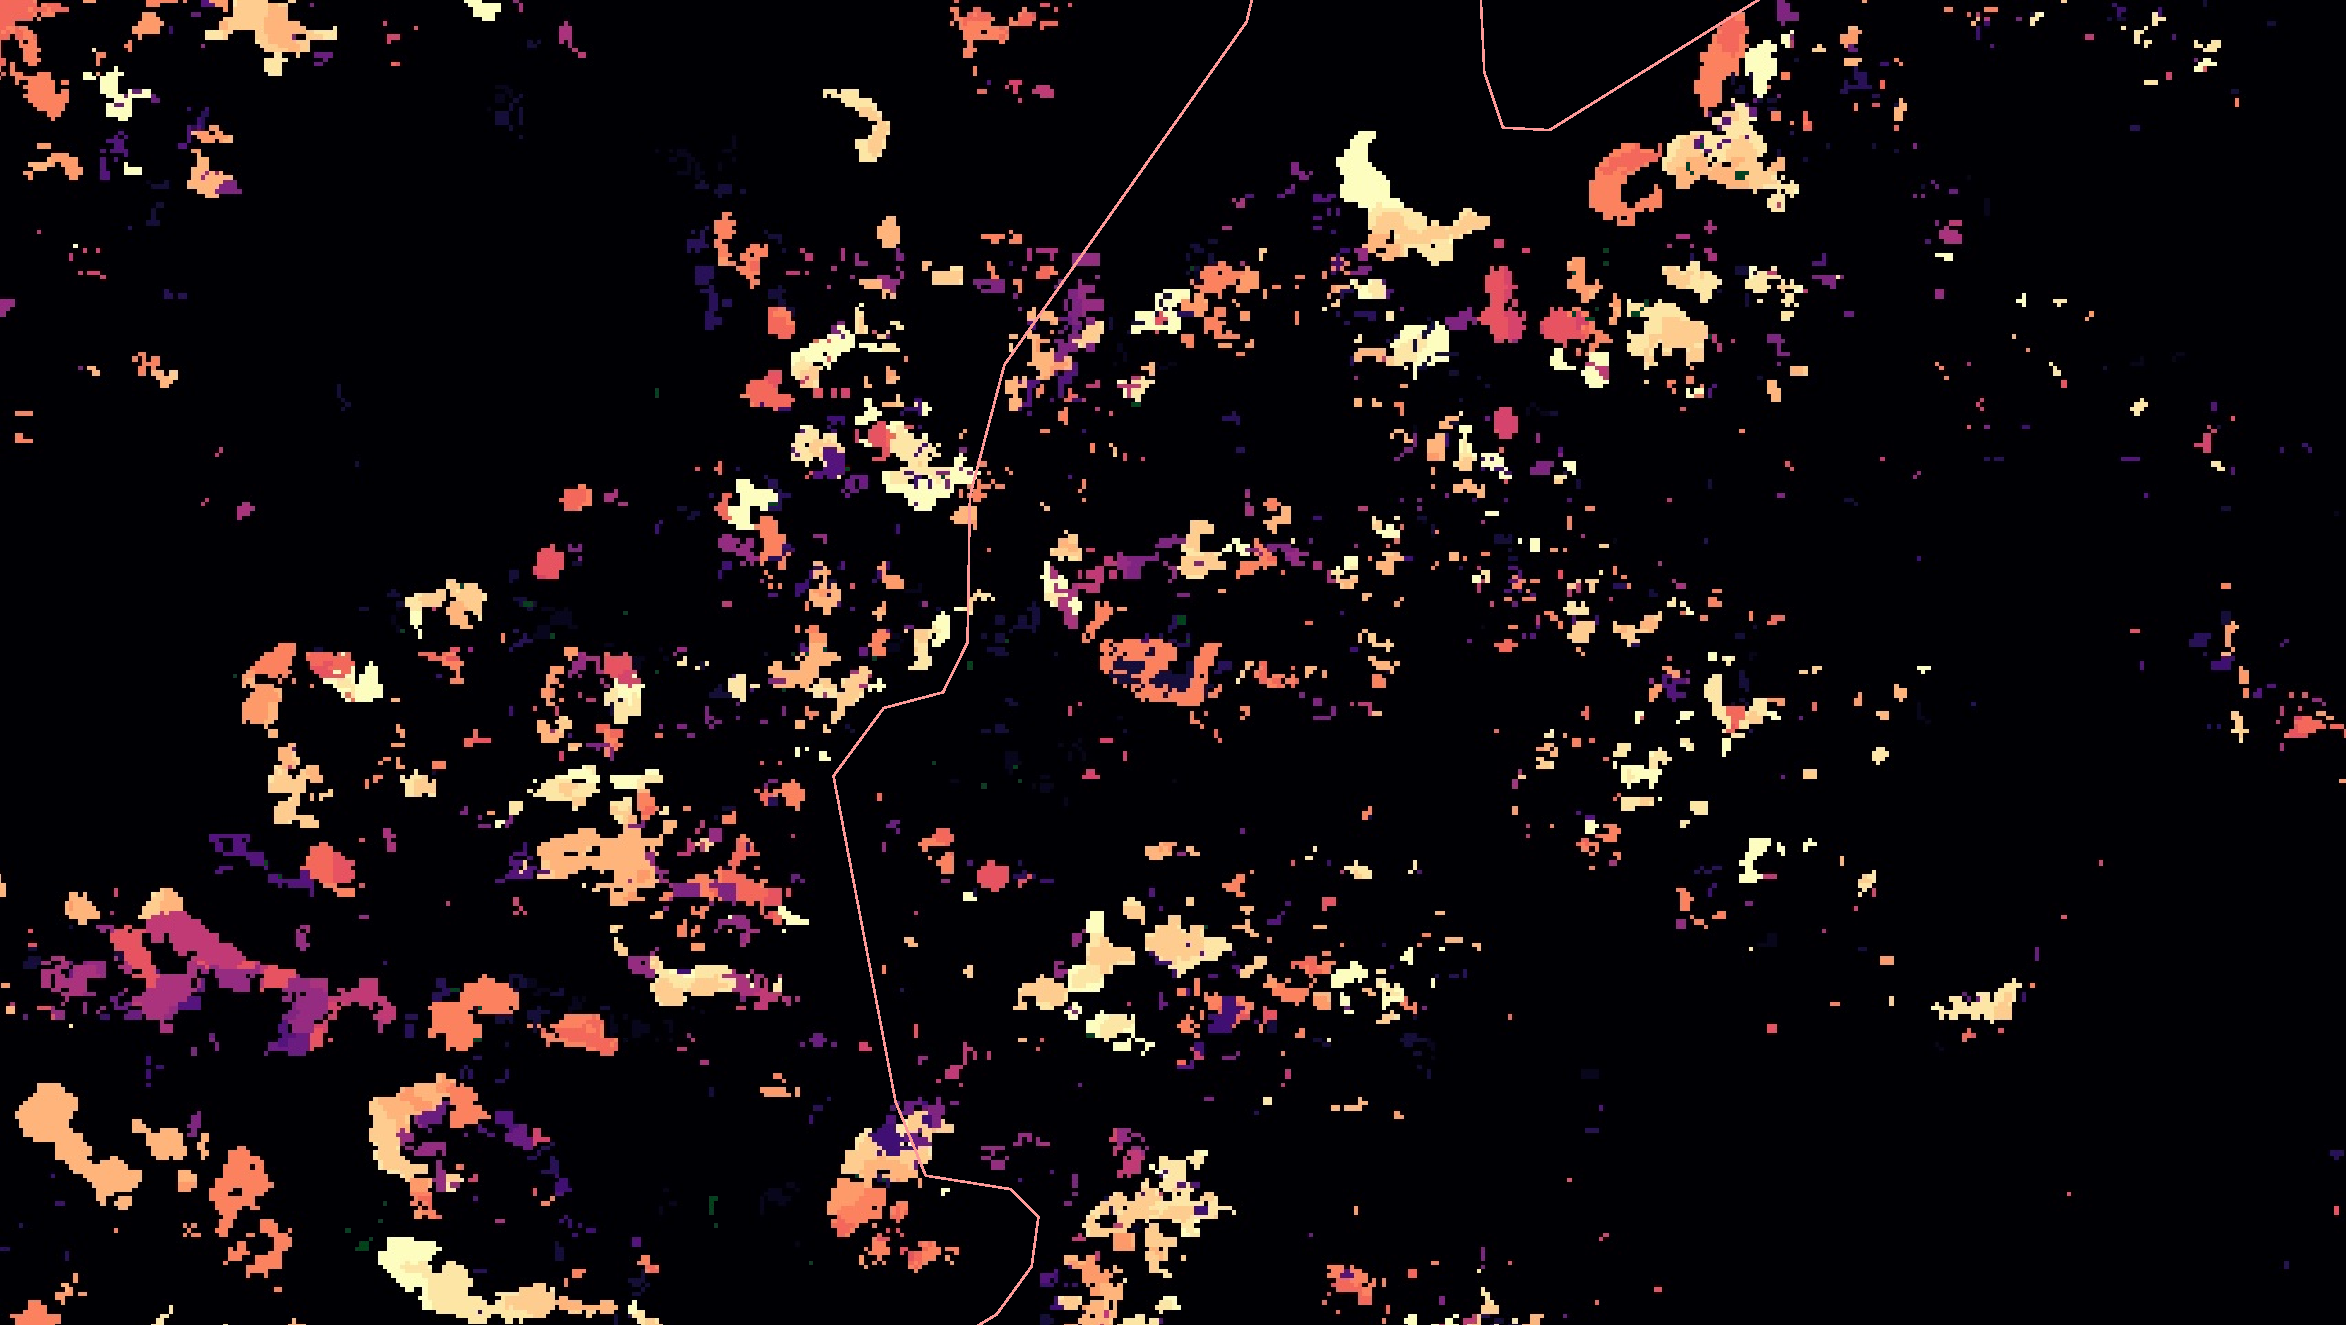
\includegraphics[width=5 in,angle=0]{Figs/loss_v_gain.pdf}}
\smallskip
\normalsize
\emph{Notes}: Forest loss (shaded red-to-yellow to indicate whether the cell was deforested in the past or recently) and gain (green) over the entire sample period (2001-2017) in southern Jharkhand, India. %Forest loss is far more common than forest gain (which are a small share; the only cells with forest gain are in dark green in the bottom left of the above figure) in the regions under consideration, although India reportedly experienced net forest-gain in the decades preceding the analysis \parencite{Foster2003-uz}
\end{minipage}
\end{center}
\end{figure}

% subsection deforestation_data (end)


\subsection{Administrative and Political Data} % (fold)
\label{sub:administrative_and_political_data}


We use the \textcite{infomap2001indiamap} geocoded village-level Indian census to get boundaries of roughly 286,000 villages across the nine states where we conduct our analysis. For each village, we aggregate the pixel-level deforestation data described above to the village level. To do this, we first compute zonal statistics for each village, which entails merging the pixel level raster dataset with the village polygons and counting the number of cells corresponding with each deforestation year in each village.  We then convert the number of deforested cells per year into hectares--a commonly used unit when discussing medium-scale areas--by multiplying the number of deforested cells in each year by $0.09$, since a hectare is $10,000 m^2$ and the area of a LANDSAT cell is $30\times30=900 m^2$. This gives us the dependent variable in terms of deforested area in hectares in each year for each village.

\subsection{Measuring Scheduled Areas} 

The construction of our treatment variable relies on manual coding of whether a village belongs to Scheduled Areas or not. To do this, we use information on the Government of India's Ministry of Tribal Affairs website. Each state releases official documents that list specific village names as Scheduled, or in cases where all villages within a block or district are Scheduled, the names of those blocks and districts are released.

To remain consistent in our coding strategy across states and avoid human error, we code an entire block as Scheduled if \emph{any} village was designated as Scheduled within the block. Empirically, this approach is conservative because, while it accurately codes Scheduled Areas when all villages in a district and block are inside the treatment area, it codes some untreated villages within a block as treated -- that is, the resulting bias will towards zero. This coding is illustrated spatially in Figure \ref{fig:schmap} and a validation exercise that compares this coding with government issued maps is presented in \textcite{gulzar2019}, Appendix B.

\begin{figure}[htbp!]
\begin{center}
\begin{minipage}{1 \linewidth}
\caption{\textbf{Forest Loss in the Study Period (Left) and Scheduled Areas (Right) in India}\label{fig:schmap}}	
\centerline{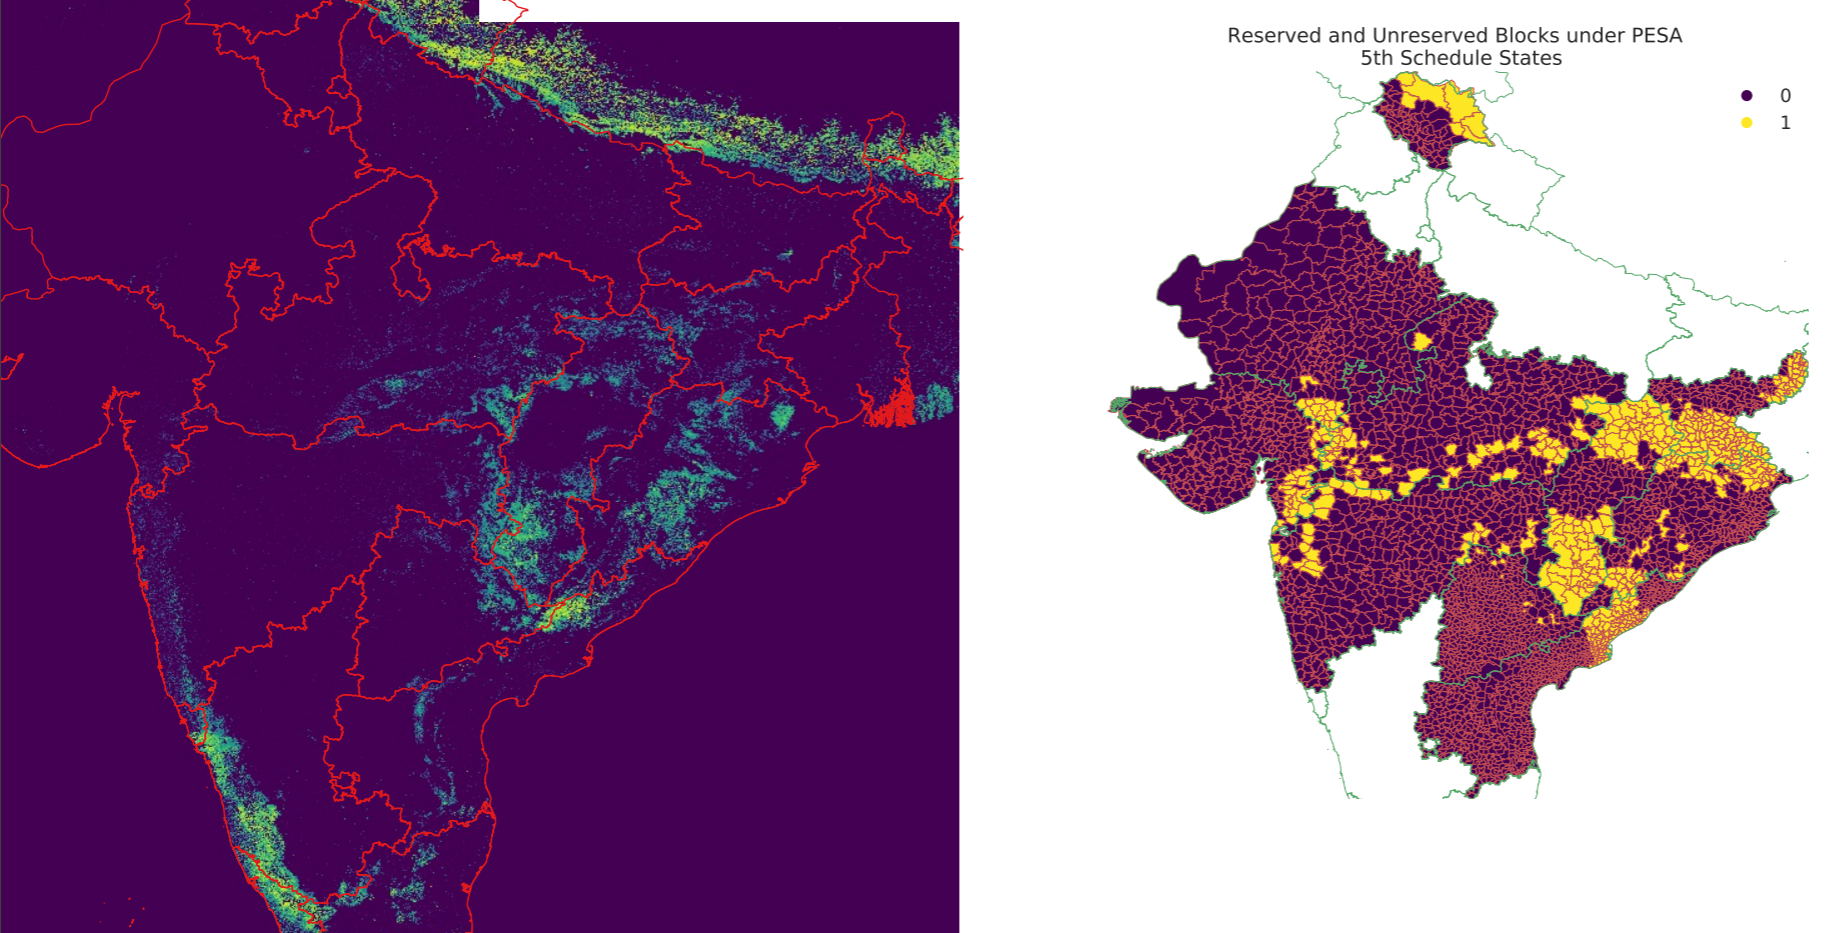
\includegraphics[width=6 in,angle=0]{Output/side_by_side.png}}
\smallskip
\normalsize
\emph{Notes}: Left panel generated using data from \textcite{Hansen2013-vk} where brighter shades correspond with more recent deforestation. Right panel reflects Scheduled Areas under the Fifth Schedule of the Indian Constitution and neighbouring regions.
\end{minipage}
\end{center}
\end{figure}

Once each village is coded as Scheduled or not according to the above procedure, we construct a switching indicator for Scheduled Areas in each state based on archival research of the first \emph{gram-panchayat} election in Scheduled Areas in accordance with PESA, where quotas were instituted for Scheduled Tribes. We illustrate this timing in Figure \ref{fig:timing}. This restricts us to estimating treatment effects for 4 of the 9 treatment states because the remaining five implemented PESA before the first year in which forest data is available, which gives us no over-time variation in their treatment status.  

We merge this village level treatment timing data with the deforestation panel to finally arrive at our analysis sample, which is a balanced panel of about 286,000 villages over 17 years. Not all of these villages have any forest cover to begin with. We subset our main analysis to villages with an ex-ante forest cover index of 2 or more out of a possible 100 in 2000 as per the GFC data in our preferred specification. This is approximately the $75^{th}$ percentile in the distribution of ex-ante forest cover, which we label as `forested' in our analysis.\footnote{While this may seem like an extreme cutoff, this is motivated by the fact that over 50\% of the villages in our sample have an average forest index of 0.07 out of 100.} We analyse the sensitivity of our estimates to this cutoff.

\begin{figure}[htbp!]
\begin{center}
\begin{minipage}{1 \linewidth}
\caption{\textbf{PESA Implementation Timing for Nine States} \label{fig:timing}}	
\centerline{\figinc{Output/PESA_adopt2.pdf}}
\smallskip
\normalsize
\emph{Notes}: PESA was implemented only in scheduled areas within each of these states. So, while one of the specifications uses the staggered rollout of the PESA programme, our preferred specification only uses \emph{within-state} variation in PESA treatment status to estimate the treatment effect 
\end{minipage}
\end{center}
\end{figure}

\section{Empirical Strategy} % (fold)
\label{sec:empirical_strategy}


Our objective is to study how improved political representation for ST affects deforestation outcomes. We employ a difference-in-differences design to study the effect of the roll out of PESA on deforestation, where the first difference is between Scheduled Areas and non-Scheduled Areas, and the second is the onset of the first post-PESA election in Scheduled Areas. In Scheduled Areas, political representation for ST is stronger through both the introduction of panchayat elections (\emph{after} PESA) and a substantial and persistent ST quota in the entire geographic area. Non-Scheduled Areas have had local government since the introduction of the 73rd amendment.\footnote{Except for the state of Jharkhand that we discuss in Section \ref{jharkhand}.} In addition, some villages in these areas are reserved for candidates who identify as ST, SC, OBC, and/or as women based on the proportion of the group's population in the local area, a reservation that rotates over election cycles. Critically, the rotating quotas, only reserve a given area until the next five-year election, unlike in Scheduled Areas, where the quota remains in perpetuity.\footnote{\textcite{dunning2013ethnic} argue that the rotating nature of the quota is an important impediment towards its efficacy. For more details on the rotating quota system in non-Scheduled Areas see \textcite{chattopadhyayWomenPolicyMakers2004, bhavnani2009electoral,jensenius2017social}.} Therefore, what we estimate using a difference-in-differences design can be interpreted as the differential effect of increased representation for ST.

%Because we compare non-Scheduled Areas, where a fraction of local councils are reserved, with Scheduled Areas, where all councils are reserved, the treatment effect we estimate can be thought of as a lower bound of the effect of increasing ST representation on deforestation. 

%Therefore, what we estimate using a difference-in-differences design we describe below,  can be interpreted as the differential effect of panchayat institutions when augmented with quotas.

% As a result, we can think of treated villages (in Scheduled Areas and after a PESA election), as receiving the bundled treatment of local elections as well as a 100\% reservation of seats for ST candidates


%% Isn't it as simple as this:
% Treated = elections + 100% quota
% Control = elections + rolling quotas by population share

% I would say "bundled" rather than "two treatments"
% Also SA and non-SA, rather than PESA and non-PESA

%Recall that the introduction of PESA into Scheduled Areas in the nine states under consideration introduced (A) elected village representatives to the panchayats in each village and (B) quotas for Scheduled Tribes in these panchayats. These can be thought of as two components of our treatment of increased representation for the Scheduled Tribes that were contemporaneously introduced in Scheduled Areas. Note that non-Scheduled Areas had already been treated with (A) since the introduction of elected panchayats through the 73rd amendment in 1993. What we estimate using a difference-in-differences design we describe below, therefore, is a comparison between non-Scheduled Areas already `treated' with \emph{A} and Scheduled Areas that are newly treated with \emph{A and B}. This can be interpreted as the differential effect of panchayat institutions when augmented with quotas.\footnote{We have substantive reasons to believe that the two treatments A and B are complementary (that is, their effects are multiplicative), so the `joint' effect is of interest. Furthermore, the effect we estimate can be thought of as a lower bound because rotating quotas exist for identity categories in non-PESA areas as well \parencite{dunning2013ethnic}.}

Since we have a panel dataset of each village with time-varying binary treatment, we begin the analysis with a two-way fixed-effects estimator:

\begin{equation}\label{base}
Y_{ist} = \tau \text{Scheduled Area}_{is} \times
\text{PESA Election Year}_{ist} +  \delta_i + \gamma_t +  \epsilon_{ist}
\end{equation}

where $i$ indexes villages, $s$ indexes state, and $t$ indexes years. $Y_{ist}$ is the total area (in Hectares) deforested in village $i$ in year $t$ , Scheduled Area $\times$ PESA Election Year$_{it}$ is a dummy that for villages in scheduled areas in the year the first election where PESA was implemented, $\delta_i$ is a village fixed effect, and $\gamma_t$ is a year fixed-effect.\footnote{Note that village fixed effects account for \emph{all time invariant village characteristics}, such as geographical variables, or slow-moving socio-demographic ones such as ethnic composition. It also means that the base term for Scheduled Areas cannot be included in the regression because of perfect collinearity.} $\tau$ corresponds with the effect of the introduction of PESA elections in Scheduled Areas. This estimator includes village and year fixed effects which account for village-level unobserved characteristics that can directly affect deforestation rates, as well as common shocks (such as a national policy, such as the Forest Rights act, or a national decline in economic activity following the recession) that might affect deforestation rates. We cluster standard errors by village in the main tables and examine robustness to more aggregated clustering, with the latter intended to account for potential spatial spillovers and to be consistent with the assignment unit.  

The difference-in-differences design relies on the assumption of parallel trends, which in this context means that villages that fall in Scheduled Areas were on the same deforestation trajectories from those that were not in Scheduled Areas before the introduction of local elections under PESA. One might reasonably worry that this assumption might not be valid, and that simple village fixed effect, tantamount to having a single village-level intercept, may not capture potential time-varying confounding. To account for this, we also introduce village level linear time trends. These trends remove variation from the outcome by village that may potentially mis-attribute treatment effects to the policy if take-up was indeed non-random and related to the underlying village time trend of deforestation. Specifically, we estimate specifications of the following form:

\begin{equation}\label{ttrend}
Y_{ist} = \tau \text{Scheduled Area} \times \text{PESA Election Year}_{ist} +
\delta_i + \gamma_t + \delta_it + \epsilon_{ist}
\end{equation}

where we have added additional $\delta_i t$  village-specific linear time trends. In this specification, $\tau$ is identified off within-village variation, conditional on common year level unobservables \emph{and} village-level time trends for the entire sample. These village-specific time trends address confounding that might arise from secular changes in deforestation rates \emph{within any given village}; say, if a village has been steadily deforesting over time. 

One might reasonably worry that different state-level policies adopted at particular times may constitute a plausible time-varying confounder, which renders the estimate from the common year-fixed-effects specification biased. In particular, the Forest Rights Act (passed in 2006, implemented in 2008), which delegated various forest-related rights to the village panchayats \emph{regardless of their PESA status} was implemented unevenly across different states, and therefore a common year-fixed-effect might not account for this confounding. 
More concretely, since PESA was implemented more strongly in Odisha relative to all other states \parencite{Patnaik2007-ku}, a common intercept for 2008 might not account for this appropriately. We therefore introduce, state $\times$ year Fixed-effects, which account for time-varying state-level confounders, such as the FRA. To do so, we run the following regression:

\begin{equation}\label{styfe}
Y_{ist} = \tau \text{Scheduled Area} \times \text{PESA Election Year}_{ist} +
\delta_i + \gamma_t + \xi_{st} + \epsilon_{ist}
\end{equation}

where $\xi_{st}$ is a vector of state-year fixed effects. These fixed effects accounts for confounders that vary by state for each year and isolate the effect of PESA by comparing scheduled areas and non-scheduled areas \emph{within} each state, holding state policy constant for each year. In other words, this analysis pools across differences-in-differences estimates (wherein the treatment and control units are \emph{within} each state), and does not rely on the staggered adoption of the policy for causal identification. This specification yields estimates of the average treatment effect on the treated (ATT) even when treatment effects are heterogeneous, which the standard two-way FE model does not \parencite{Imai2019-kp}.
The state-year FEs restrict identifying-variation to within-state difference-in-differences for four states (Chhatisgarh, Jharkhand, Odisha, and Maharashtra) that have variation in PESA implementation in our sample. Finally, we add back village time trends to address secular trends in deforestation at the village level. This is, to our mind, the most credible comparison wherein parallel trends are likely to hold.

\begin{equation}\label{styfett}
Y_{ist} = \tau \text{Scheduled Area} \times \text{PESA Election Year}_{ist} +
\delta_i + \gamma_t + \xi_{st} + \delta_i t + \epsilon_{ist}
\end{equation}

% section empirical_strategy (end)

% ########  ########  ######  ##     ## ##       ########  ######
% ##     ## ##       ##    ## ##     ## ##          ##    ##    ##
% ##     ## ##       ##       ##     ## ##          ##    ##
% ########  ######    ######  ##     ## ##          ##     ######
% ##   ##   ##             ## ##     ## ##          ##          ##
% ##    ##  ##       ##    ## ##     ## ##          ##    ##    ##
% ##     ## ########  ######   #######  ########    ##     ######

\section{Results}\label{sec:Results} % (fold)

\subsection{Visualizing the data}
As a first cut of our empirical approach, we visualize average (residualized) deforestation rates in Scheduled and non-Scheduled Areas for each year before and after PESA implementation (constructed relative to the year of implementation in each state) in Figure \ref{fig:schtrends}. We see that the rate of deforestation flattens substantially in scheduled areas following the implementation of the act.



\begin{figure}[htbp!]
\begin{center}
\begin{minipage}{1 \linewidth}
 \caption{\textbf{Average Deforestation in Scheduled and Control Areas Before and After the Implementation of the Panchayat Extension to Scheduled Areas Act} \label{fig:schtrends}}	
\centerline{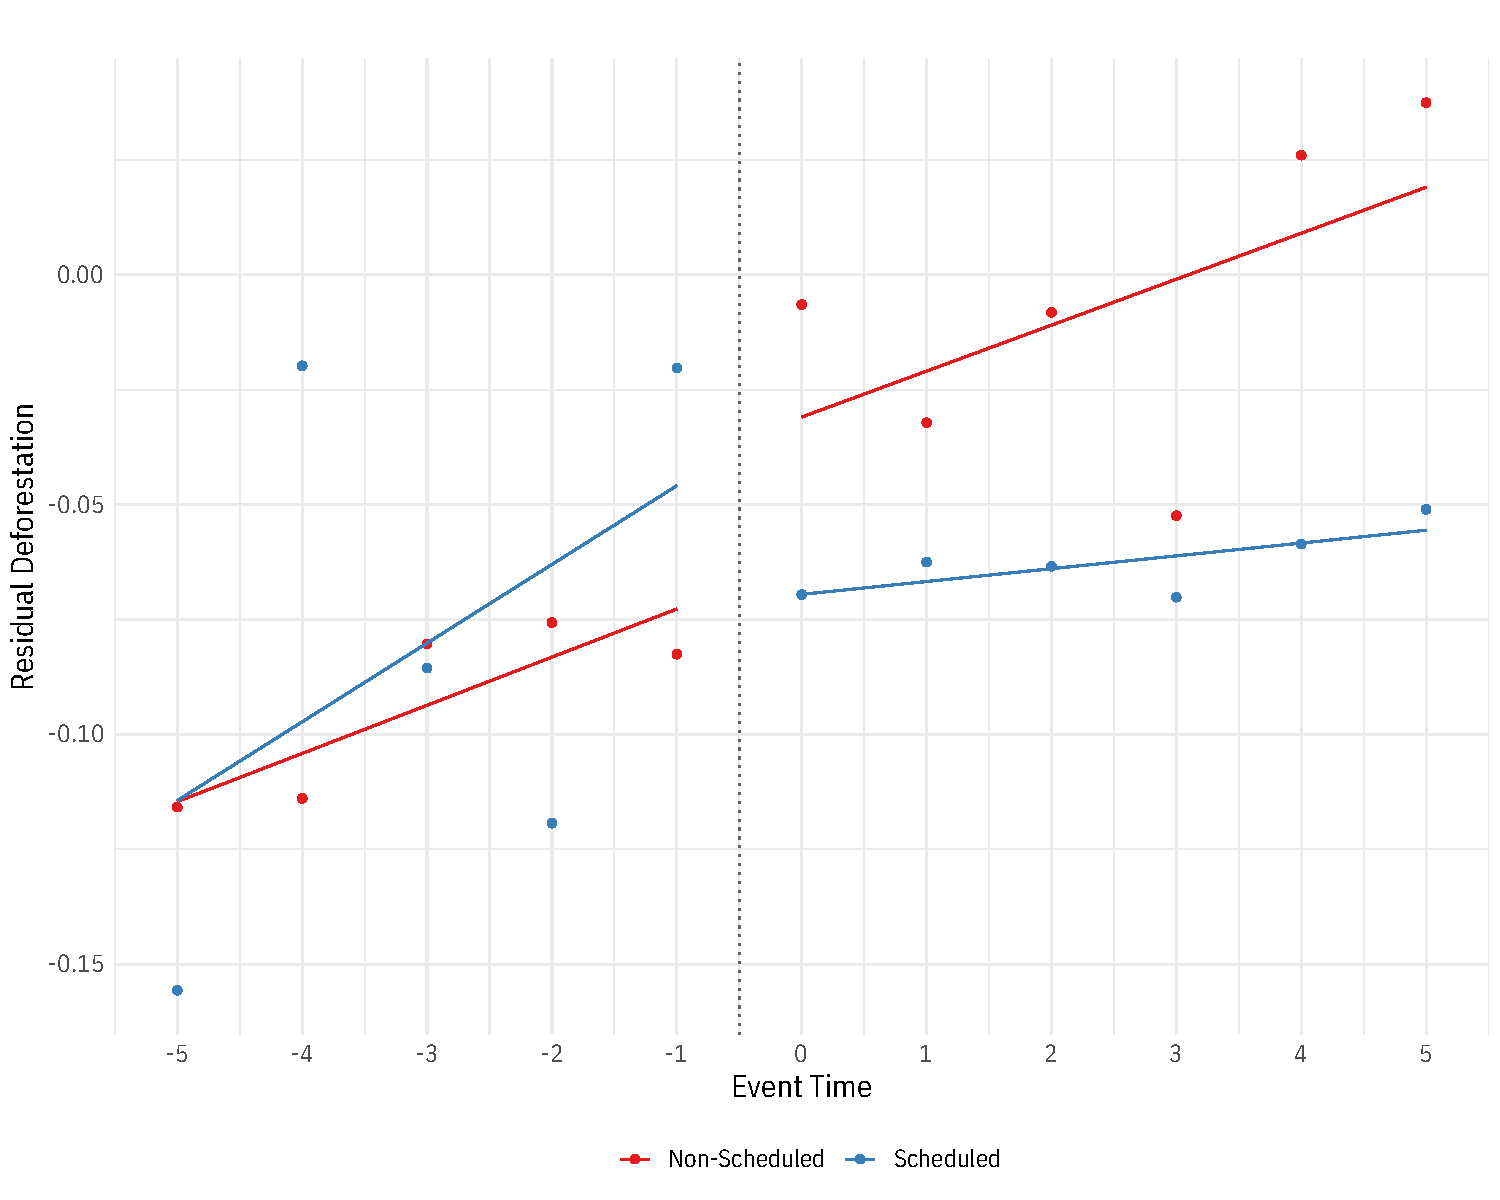
\includegraphics[width=5 in,angle=0]{Output/levels_time_trends.pdf}}
\smallskip
\normalsize
\emph{Notes}: The outcome has been residualized for group averages over the whole panel. Each dot is the average (residualized) deforestation for the treatment and control groups respectively in event time (i.e. years before the implementation of PESA in \emph{a particular state}).
\end{minipage}
\end{center}
\end{figure}



\subsection{Main Effects\label{MainEffects}}
Our main regression findings are reported in Table \ref{table:regres} below. Column 1 reports estimates of $\tau$ from \ref{base}, column 2 reports the estimates from \ref{ttrend}, column 3 reports estimates from \ref{styfe},
and column 4 reports results from \ref{styfett}. As discussed above, for our primary analysis, we subset to villages with reasonable amounts (mean index of over 2\%) of ex-ante forest cover, since including villages with effectively no forest cover mechanically biases estimates towards zero (since villages with no forest cover cannot have decreases in the rate of forestation), particularly because these are typically densely populated villages in `control' (non-scheduled) areas.


\begin{table}[!htbp] \centering 
  \caption{Main Effects (Difference in Differences)} 
  \label{table:regres} 
\begin{tabular}{@{\extracolsep{0pt}}lcccc} 
\\[-1.8ex]\hline \\[-1.8ex] 
\\[-1.8ex] & \multicolumn{4}{c}{Annual Deforestation in Hectares} \\ 
\\[-1.8ex] & (1) & (2) & (3) & (4)\\ 
\hline \\[-1.8ex] 
 Scheduled X PESA & $-$0.088$^{***}$ & $-$0.032$^{***}$ & $-$0.016$^{**}$ & $-$0.067$^{***}$ \\ 
  & (0.008) & (0.010) & (0.007) & (0.012) \\ 
 Village FE & $\checkmark$ & $\checkmark$ & $\checkmark$ & $\checkmark$ \\ 
Year FE & $\checkmark$ & $\checkmark$ &  &  \\ 
Village TT &  & $\checkmark$ &  & $\checkmark$ \\ 
State X Year FE &  &  & $\checkmark$ & $\checkmark$ \\ 
Dep. Var. Mean & 0.22 & 0.22 & 0.19 & 0.19 \\ 
N. Villages & 52776 & 52776 & 31601 & 31601 \\ 
N & 897,192 & 897,192 & 537,217 & 537,217 \\ 
\hline \\[-1.8ex] 
\multicolumn{5}{l}{$^{*}$p $<$ .1; $^{**}$p $<$ .05; $^{***}$p $<$ .01} \\ 
\multicolumn{5}{l}{Cluster-Robust Standard Errors (by village)} \\ 
\end{tabular} 
\end{table} 


We find that the estimated treatment effects are consistently large and negative. In our preferred specification with state-year fixed effects and village trends (column 4) the implied reduction in the rate of deforestation is approximately $0.06$ hectares per village per year, approximately $31\%$ on the overall mean of $0.19$.\footnote{The number of observations changes between columns 1-2 and 3-4 because columns 3-4 restrict the sample to the four treatment states because of state $\times$ year fixed effects} The implied back-of-the-envelope effect is on the order of 1440 hectares per year (see Appendix \ref{treat_size} for details.) The difference in the estimated treatment effect between the two-way fixed-effect estimate (column 1), the specification that includes additional time-trends (column 2), and state-year fixed effects (column 3) suggests that there was plausibly positive selection into treatment. The coefficients from the two specifications are in the same order of magnitude and consistently have the same sign, which gives us confidence that the time trends are absorbing confounding in terms of selection into treatment.%\footnote{Appendix Table ~\ref{table:regres_by_state} reports regression estimates separately for each state.}


% ########   #######  ########  ##     ##  ######  ########
% ##     ## ##     ## ##     ## ##     ## ##    ##    ##
% ##     ## ##     ## ##     ## ##     ## ##          ##
% ########  ##     ## ########  ##     ##  ######     ##
% ##   ##   ##     ## ##     ## ##     ##       ##    ##
% ##    ##  ##     ## ##     ## ##     ## ##    ##    ##
% ##     ##  #######  ########   #######   ######     ##

\subsection{Robustness Checks}

\paragraph*{Results are stronger for higher ex-ante forest cover.} We vary the ex-ante forest cover cutoff for entry into our estimation sample and estimate \ref{styfett}
on the subset sample to test for whether the coefficient is sensitive to the choice of ex-ante forest cutoff. The results are presented in Figure
\ref{fig:cutoff_plot}. 

\begin{figure}[htbp!]
\begin{center}
\begin{minipage}{1 \linewidth}
\caption{\textbf{Treatment Effects on Annual Deforestation as a Function of Ex-Ante Forest Cover Cutoffs}\label{fig:cutoff_plot}} 	
\centerline{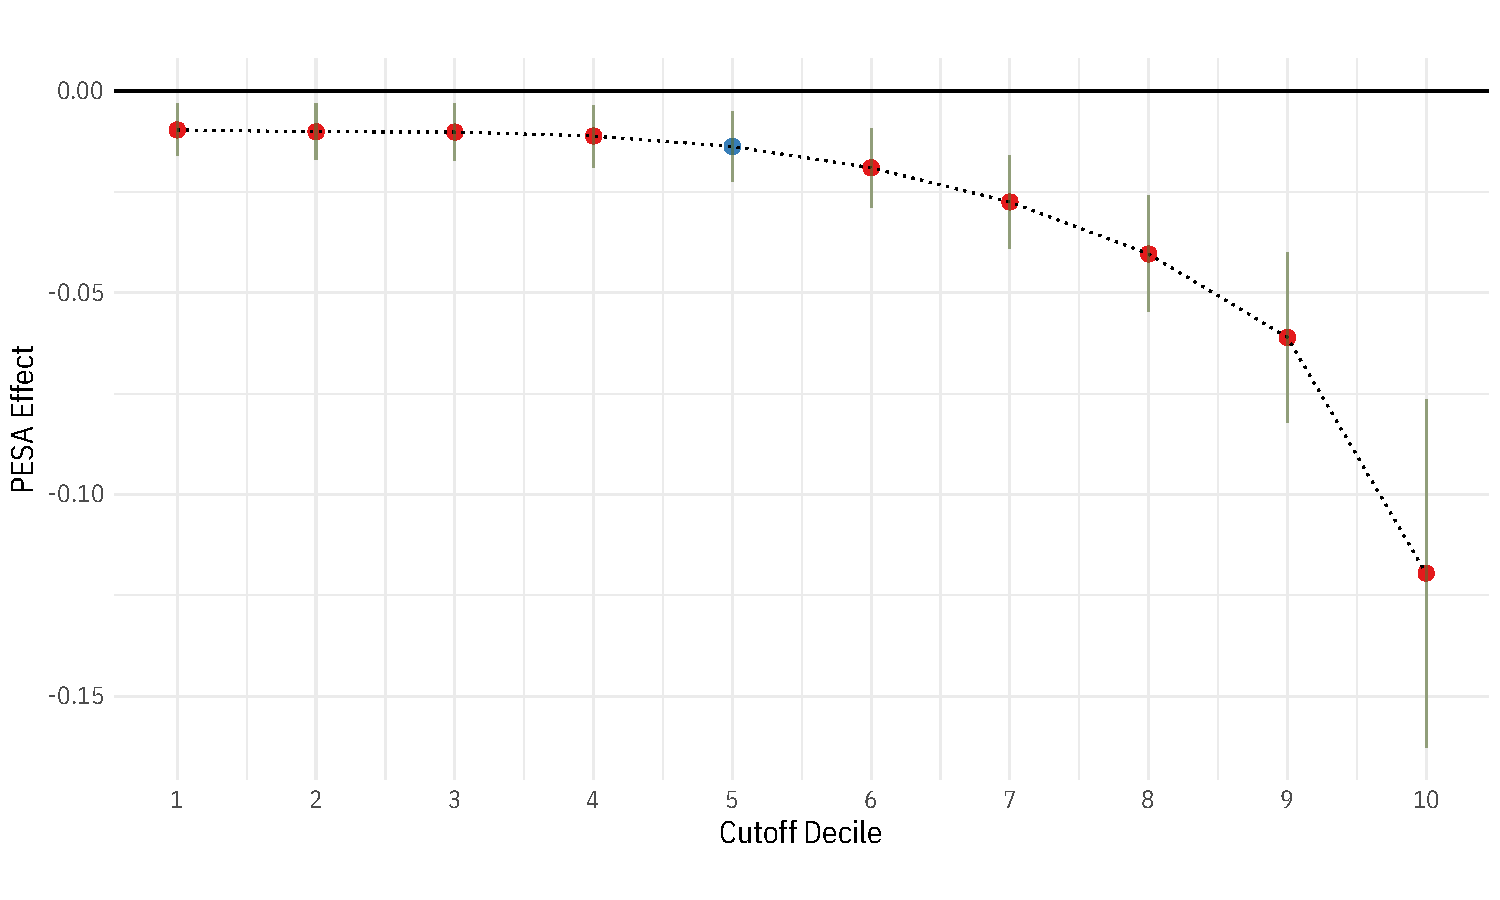
\includegraphics[width=5 in,angle=0]{Output/varying_cutoff2.pdf}}
\smallskip
\normalsize
\emph{Notes}: The figure reports treatment effect estimates with specification \ref{styfe}., with SE estimates clustered by village. The point in blue corresponds to the median cutoff. The 'forested' threshold (i.e. the threshold used to subset the data for analysis in table \ref{table:regres} is approximately at the 75th percentile.
\end{minipage}
\end{center}
\end{figure}

\paragraph*{Results are consistent with an alternative source of forest data.} We estimate the same specifications as in Section ~\ref{sec:empirical_strategy} using outcome data derived from an alternate source of forest cover data: the Vegetation Continuous Fields data \parencite{Song2018-sw} aggregated by \textcite{almn2020}. This data provides annual tree cover from 2000-2014 in the form of the percentage of each pixel under forest cover \parencite{Sexton2013-xx}. A major drawback of these data, however, is that they are derived from a different satellite with a coarser resolution than our primary data (0.05 seconds $\approx 250\times250m$ vs $30\times30m$ cells in GFC) and therefore many villages' indices are derived from a small handful of measurements. Nevertheless, the results, reported in Appendix \ref{sub:auxreg}, serve as a useful robustness check and validate our main findings.

\paragraph*{Results are consistent with more aggregated clustering.}
We report results from the main specifications clustered at the block level (which are comprised of multiple villages and gram panchayats that are the relevant administrative unit for local government institutions), to account for both spatially correlated errors and serial autocorrelation in errors. Clustering at a large administrative unit is somewhat comparable to (and often more conservative than) estimating Conley standard errors with a large bandwidth. This massively increases the standard errors in specifications with many additional parameters (such as village time trends and state-year FEs), but treatment effect in our preferred specification remains significant at the 5\% level (see Table \ref{table:regres2}).

\paragraph*{Results for PESA are quantitatively larger than those for the Forest Rights Act.}
Although the FRA was implemented uniformly among all panchayats in each state, and therefore is already controlled for by the state-by-year fixed effects in our preferred specification, one might still be concerned that the FRA was disproportionately effective in Scheduled Areas, and therefore, might be driving some of the observed effect that we attribute to PESA implementation. To test for this, we implement an event-study following the recorded implementation of FRA in 2008 with Scheduled Areas as the treatment group, and report the results in Appendix Figure \ref{fig:FRA_evstud}. We find negligible effects in the event study, which suggests that there was little difference in deforestation following the FRA implementation in 2008 in Scheduled vs Non-Scheduled villages. We therefore conclude that we are not erroneously attributing the effects of the Forest Rights Act to PESA implementation, and that PESA had a clearly large effect on reducing deforestation in scheduled villages relative to the FRA.

\subsection{Event study: Impacts appear after the Introduction of PESA} % (fold)
\label{sub:dynamic_treatment_effects}

To examine whether PESA is indeed the driver of effects, we report yearly treatment effects separately for each year. Intuitively, if parallel trends hold, effects of treatment leads should be relatively insignificant and moderate in size, while the contemporaneous and lagged effects ought to be large. To do this, we estimate the following model:

\begin{equation}\label{granger}
 Y_{ist} = \delta_i + \xi_{st} +
\sum_{\phi=-1}^m \tau_{-\phi}
D_{i, t - \phi} + \sum_{\phi=0}^q \tau_{+\phi} D_{i,t+\phi}
+ \epsilon_{ist}   
\end{equation}

 which includes leads and lags of the treatment dummy to decompose the treatment effect by each year preceding and following the switch from pre- to post-PESA. We take the year immediately preceding the treatment as the omitted baseline year of comparison to avoid saturating the model.
 %\parencite[Appendix G]{cengiz2019effect}. 
 
 The results are reported graphically in Figure \ref{fig:autor_plot} for different sub-samples of the data, in increasing order of ex-ante forest levels, with the bottom left (6th decile and up) panel corresponding with the main analysis sample in the previous section.  We observe some anticipation effects (based on the significant negative coefficient for $-2$), as can be expected from a publicly announced policy, but the bulk of effects are large and persistent following the treatment year. Finally, consistent with Figure \ref{fig:cutoff_plot}, the treatment effects are larger when we restrict the sample to higher ex-ante forest cover.

\begin{figure}[htbp!]
\begin{center}
\begin{minipage}{1 \linewidth}
\caption{\textbf{Dynamic Treatment Effects of PESA Adoption on Annual Deforestation} \label{fig:autor_plot}} 	
\centerline{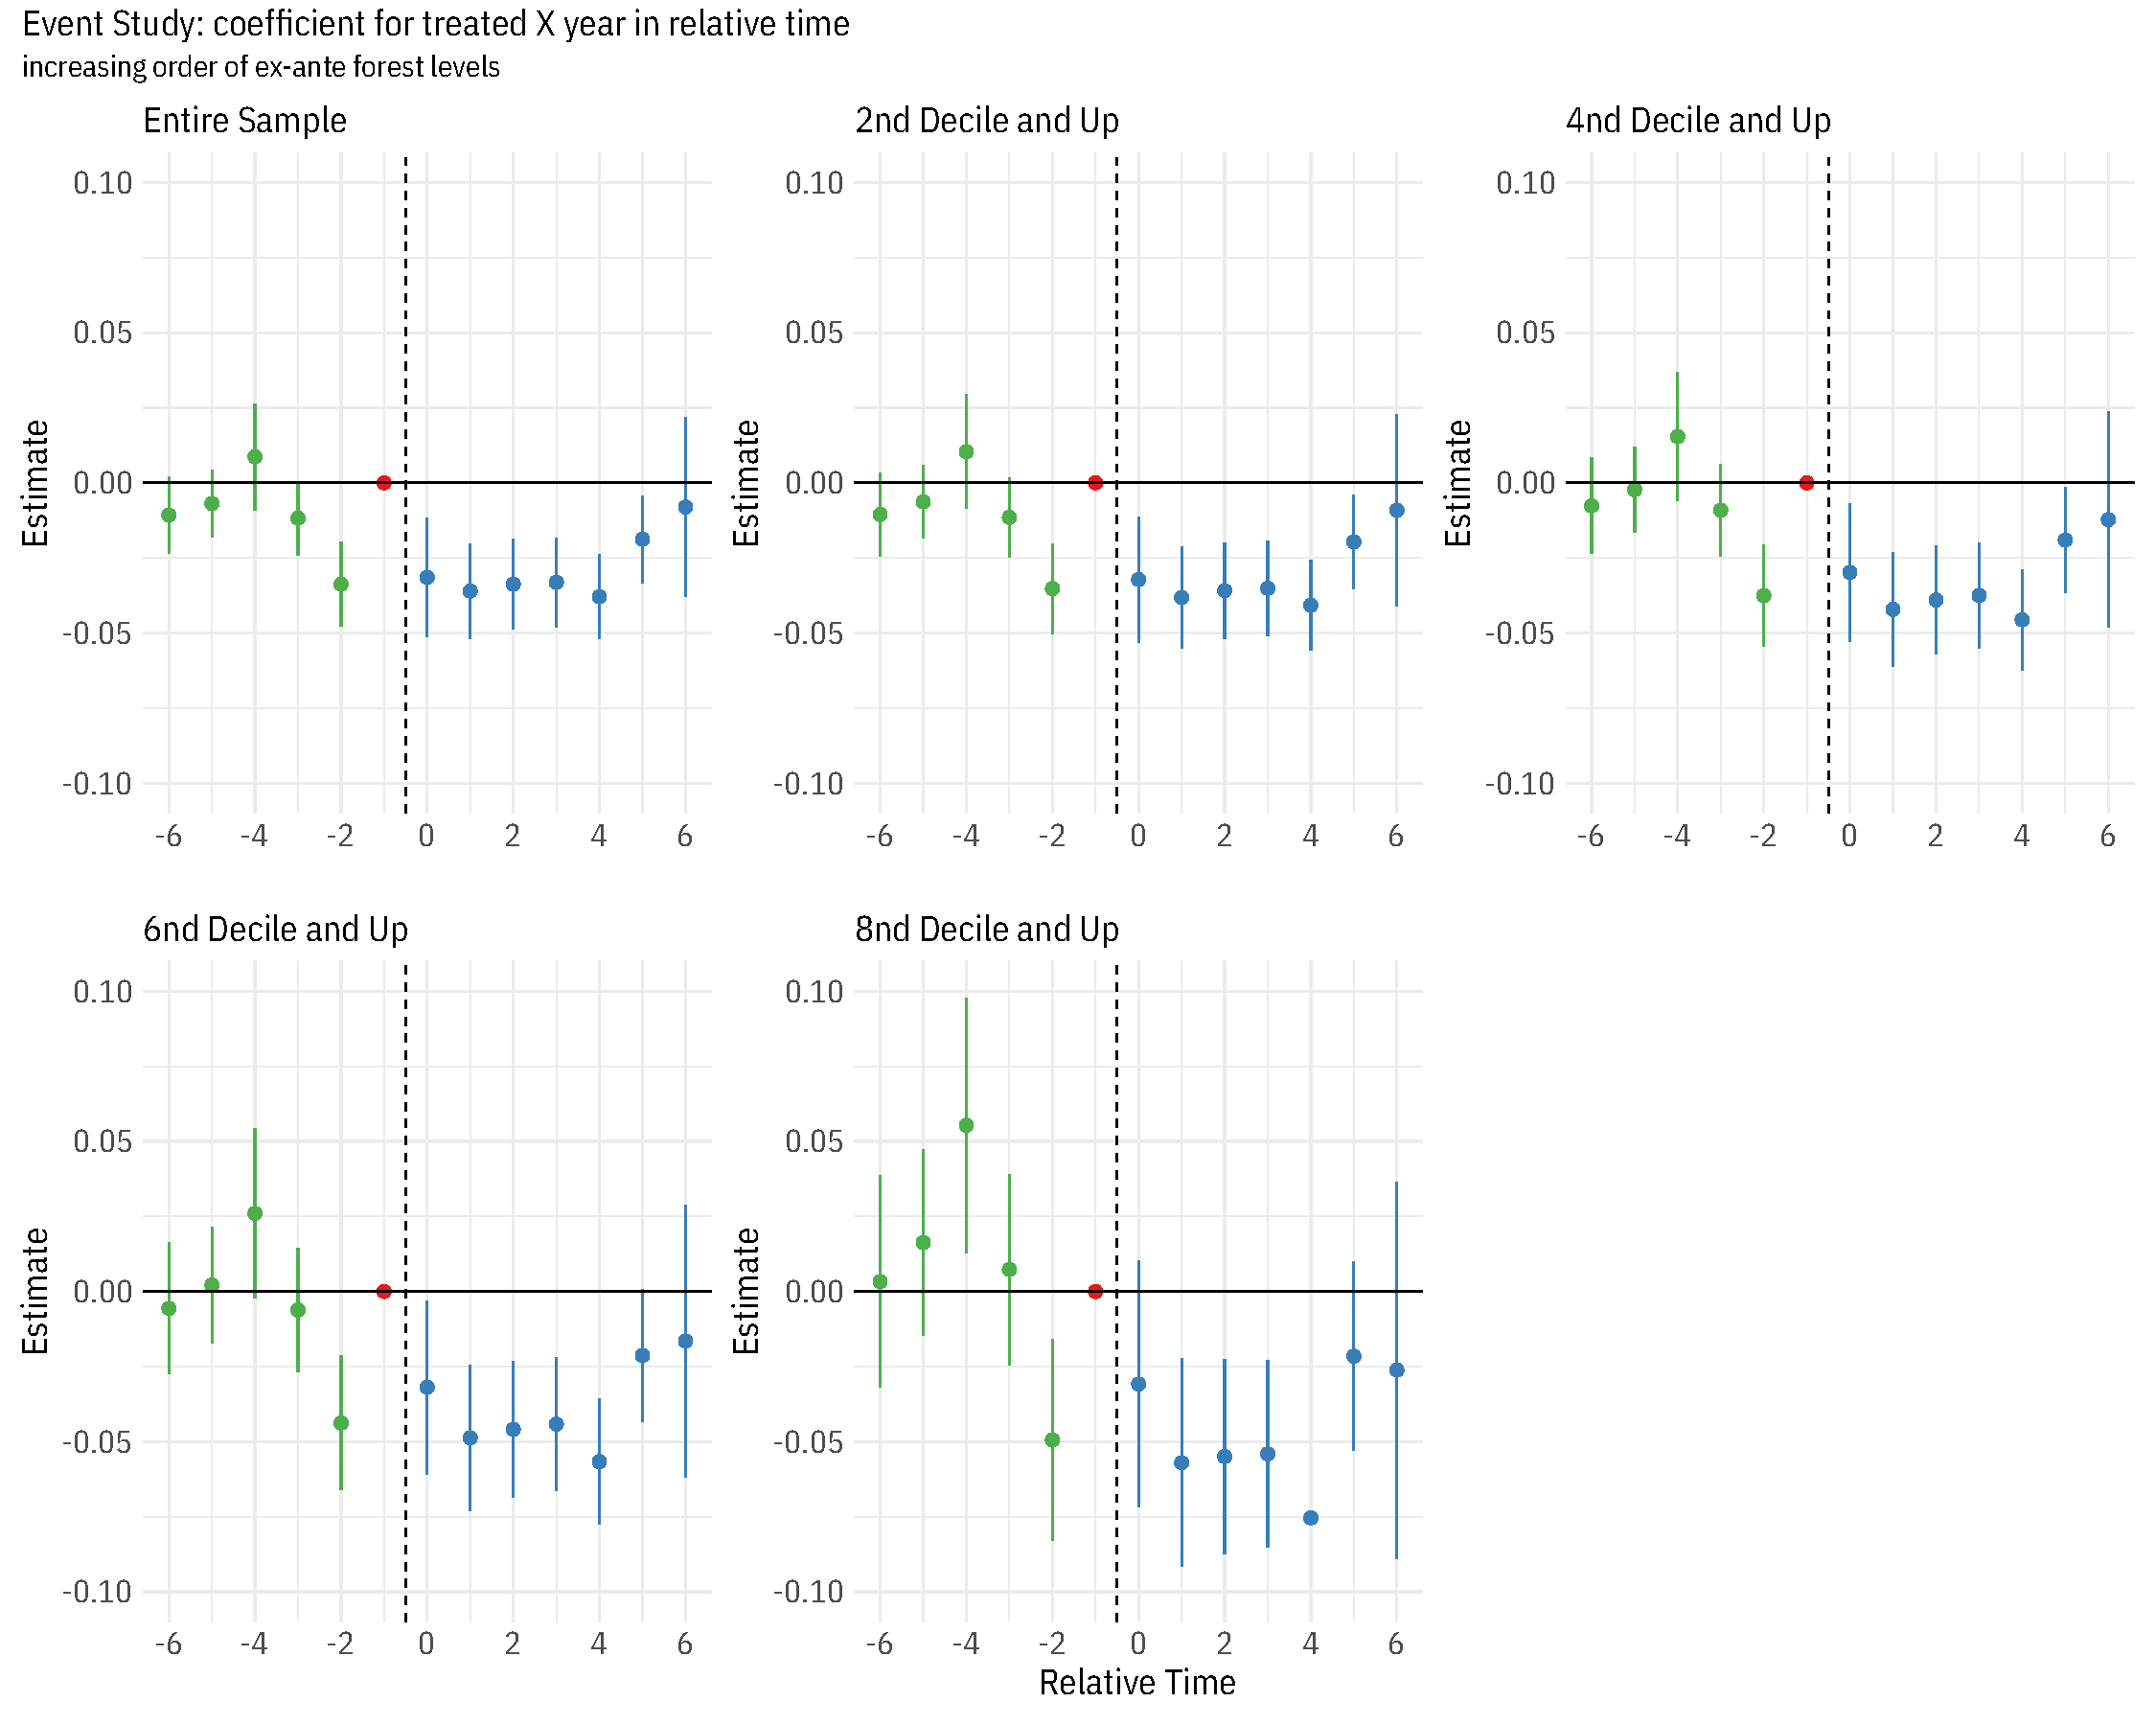
\includegraphics[width=7.5 in,angle=0]{Output/Dyn_treat_eff_big.pdf}}
\smallskip
\normalsize
\emph{Notes}: This figure presents result from the event study regression omitting time $-1$, such that each coefficient reports the difference with respect to $-1$. Standard errors are clustered by village.
\end{minipage}
\end{center}
\end{figure}


To further account for potential differences in pre-trends across the two groups, we perform a matched difference-in-differences analysis wherein we exact-match on State and ex-ante forest cover decile and coarse match on the outcome variable (deforestation area) for the villages in our sample, as suggested by \textcite[]{Imai2019-kp}. This allows us to estimate treatment effects on the matched sample which we report in Figure \ref{fig:panelmatch}. This analysis restricts the sample to treatment and control villages that are in the same state, have comparable amounts of ex-ante forest cover in 2000 (that is, they are in the same decile for ex-ante forest cover), and have a similar rate of deforestation for 4 years prior to PESA implementation (which mechanically rules out differential pre-trending by sub-setting to the best match to treatment villages). We report a balance-test for pre-treatment deforestation in Figure \ref{fig:panelmatchbal} and conclude that the matched samples are well-balanced (with the comparison in SD motivated by \textcite[]{imbens2015causal}, who argue that standardised balance tests are advisable over comparisons in raw measures).

In summary, after adjusting for pre-trends using panel-matching, we find that the treatment effect appears in the election year, persists for a few years, and is consistently large and negative. This provides stronger evidence to justify a causal interpretation of the observed decline in deforestation rate following the introduction of PESA. 

%It is worth noting that the data suggest that after about a five year period, treatment effects revert to zero. We do not have enough data at present to continue to see if this is a one-off change or if this pattern holds for a few more years. However, there are reasonable arguments for why we see the treatment effect revert to after a few years. First, it could be the case that at the end of the first term of locally elected councils who serve for five years, local elite interests are able to co-opt the process of reelection or strike new deals that dull the efficacy of the institution. Second, it is worth remembering that while treatment reduces deforestation, on average areas are still getting deforested. With a low base of forest cover, there could be some floor effects on the degree to which the treatment is likely to continue making a difference. We leave the precise adjudication of long term effects to future work.


\begin{figure}[htbp!]
\begin{center}
\begin{minipage}{1 \linewidth}
  \caption{\textbf{Dynamic Treatment Effects of PESA Adoption on Annual Deforestation using Matched Villages}}
  \label{fig:panelmatch}	
\centerline{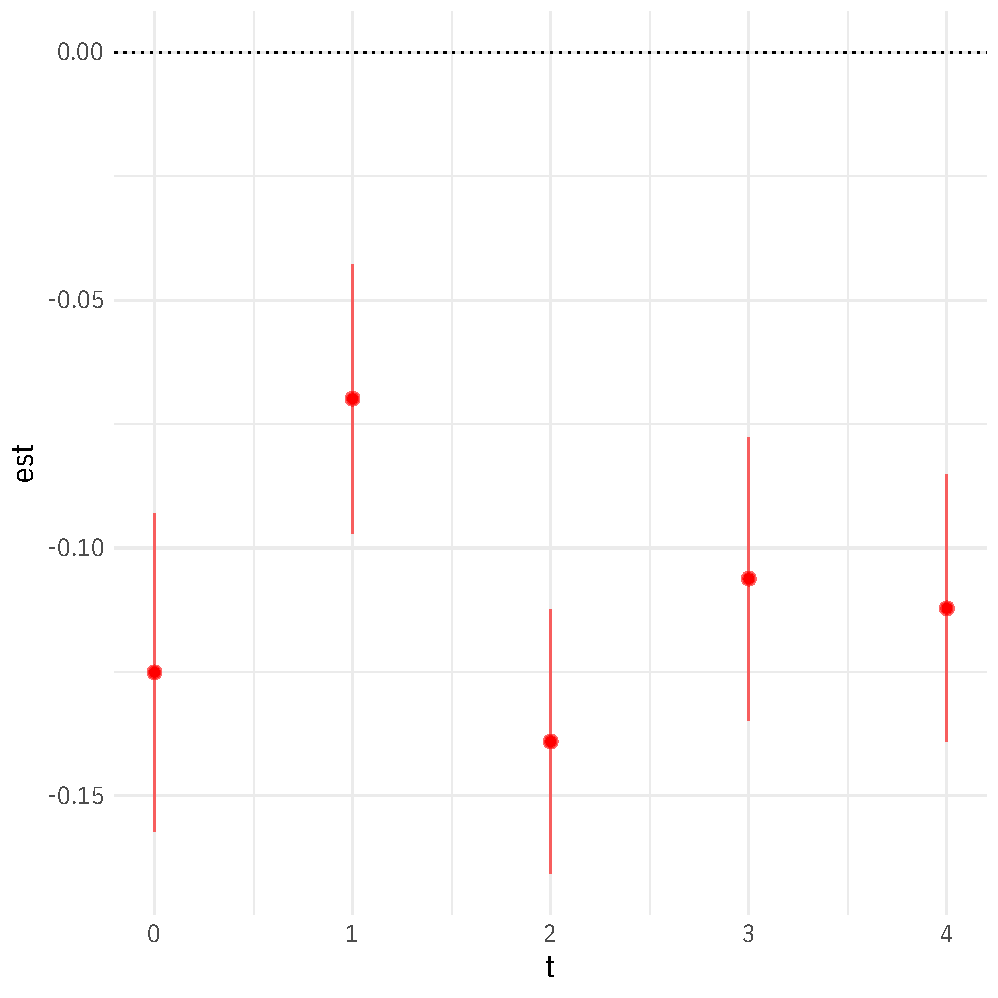
\includegraphics[width=3 in,angle=0]{Output/panelmatch_fig.pdf}}
\smallskip
\normalsize
\emph{Notes}: This figure reports results from a matched sample. We used exact matching on state and ex-ante forest decile and coarse matched on deforestation (outcome) on the 4 preceding periods to PESA implementation. Matching is performed using \texttt{PanelMatch}. Standard errors are cluster-bootstrapped by village.
\end{minipage}
\end{center}
\end{figure}


% section robustness_checks (end)

\section{Mechanisms\label{mechanisms}}

\subsection{Mining and Representation} % (fold)

One critical cause of deforestation involves the legal and illegal extraction of natural resources, whereby politicians and bureaucrats work hand-in-hand with corporate interests \parencite{Burgess2012-hk}. While researchers have shown state actors and corporate interests regularly appropriate land without local government consultation, contemporary studies of rural India have similarly shown villagers - working through their locally elected, council chairpersons, attempt to contest mining, and other large development operations \parencite{RupeeFund}. While the challenge for these villagers confronting corporate interests is substantial, our research design leverages a dramatic boost to local representation, providing an avenue by which representation may disrupt the connection between government leaders and corporate mining interests. Specifically, local representation may do so by (a) bolstering the power of local government actors and (b) electing new local leaders to power. 

As discussed in Section \ref{mining} above, Indian mining companies have worked with state actors to clear forests and exploit mineral resources, often leading to the displacement of ST and other rural inhabitants. If this mechanism is proposed operative, the PESA treatment will disrupt existing political leader - corporate mining relations, much of it at the district or state level, empowering village governance, and better aligning the preferences of ST villagers and their leaders with the preservation of forest resources. There are two observable implications of this proposed mechanism we can test directly: (1) Villages near mines should exhibit higher deforestation rates prior to PESA, and (2) PESA villages near mines, or multiple mines, should exhibit lower rates of deforestation post-PESA.


To test this, we use data from the Indian Mining Census, compiled by \textcite{asher2019rent}. The mining census lists every known mine's location and type (see Figure \ref{fig:mine_map}), which allows us to compute the distance from every village to every mine. We then use the minimum of these distances as a mediator for the regression, to examine if treatment effects are stronger for villages that are located close to mining sites. We decompose the treatment effect by tercile of distance to the closest mine in the first 4 columns in Table \ref{table:regresmine}, by every 5 km bin in Figure \ref{fig:mining_plot}, and separately for villages within $5$ km in column 5.\footnote{For completeness, we report the treatment effect decomposed by distance to every mine type with sufficient data in Appendix Figure \ref{fig:mine_het_te}.}

Consistent with the first observable implications described above, we find that villages within 5 km of a mine are experienced higher deforestation rates before PESA was implemented (see Panel A of Figure \ref{fig:mining_plot}). Consistent with the second implication, we find in both specifications, the treatment effect is strongest for villages that are close to mines, particularly those within 5 km of a mine. In addition to studying treatment effect by proximity to \emph{a} mine (the extensive margin), we also examine the effects of mining density (the intensive margin), which we define as the number of mines within a 5 km radius of each village. As shown in Table \ref{table:reg_mine_density}, we find that the treatment effect size grows within PESA villages as the number of mines increases. This points to an additional potential mechanism -- mining firms in areas with many other mines plausibly face a collective action problem in buying off local politicians, and therefore net effects on deforestation are largest in such areas. Taken together, these results suggest that both the increased power local government actors and new ST leaders are able to curb mining-induced deforestation. 


\begin{table}[!htbp] \footnotesize \centering 
  \caption{Treatment Effects on Annual Deforestation by Distance to Nearest Mine. } 
  \label{table:regresmine} 
\begin{tabular}{@{\extracolsep{0pt}}lccccc} 
\\[-1.8ex]\hline \\[-1.8ex] 
\\[-1.8ex] & \multicolumn{5}{c}{Annual Deforestation in Hectares} \\ 
\\[-1.8ex] & (1) & (2) & (3) & (4) & (5)\\ 
\hline \\[-1.8ex] 
 Scheduled $\times$ PESA $\times$ 1st Tercile & $-$0.093$^{***}$ & $-$0.043$^{***}$ & $-$0.025$^{**}$ & $-$0.079$^{***}$ &  \\ 
  & (0.010) & (0.014) & (0.010) & (0.015) &  \\ 
  Scheduled $\times$ PESA $\times$ 2nd Tercile & $-$0.103$^{***}$ & $-$0.034$^{**}$ & $-$0.026$^{**}$ & $-$0.077$^{***}$ &  \\ 
  & (0.012) & (0.016) & (0.011) & (0.016) &  \\ 
  Scheduled $\times$ PESA $\times$ 3rd Tercile & $-$0.052$^{***}$ & $-$0.004 & 0.018 & $-$0.031 &  \\ 
  & (0.017) & (0.026) & (0.017) & (0.025) &  \\ 
  Scheduled $\times$ PESA &  &  &  &  & $-$0.061$^{***}$ \\ 
  &  &  &  &  & (0.012) \\ 
  Scheduled $\times$ PESA $\times$ Mine within 5 km &  &  &  &  & $-$0.052$^{**}$ \\ 
  &  &  &  &  & (0.020) \\ 
 Village FE & $\checkmark$ & $\checkmark$ & $\checkmark$ & $\checkmark$ & $\checkmark$ \\ 
Year FE & $\checkmark$ & $\checkmark$ &  &  &  \\ 
Village TT &  & $\checkmark$ &  & $\checkmark$ & $\checkmark$ \\ 
State $\times$ Year FE &  &  & $\checkmark$ & $\checkmark$ & $\checkmark$ \\ 
Dep. Var. Mean & 0.22 & 0.22 & 0.22 & 0.22 & 0.22 \\ 
N. Villages & 52776 & 52776 & 52776 & 52776 & 52776 \\ 
N & 897,192 & 897,192 & 897,192 & 897,192 & 897,192 \\ 
\hline \\[-1.8ex] 
\multicolumn{6}{l}{$^{*}$p $<$ .1; $^{**}$p $<$ .05; $^{***}$p $<$ .01} \\ 
\multicolumn{6}{l}{Cluster-Robust Standard Errors (by village)} \\ 
\multicolumn{6}{l}{Terciles are defined based on the distribution of village distances to mines,} \\
\multicolumn{6}{l}{ with the 1$^{st}$ being $1-33$ percentile, and so on.}
\end{tabular} 
\end{table} 





\begin{figure}[htbp!]\label{fig:mining_def}	
\caption{\textbf{Deforestation and Proximity to Mining\label{fig:mining_plot}}}
\begin{minipage}{0.45 \linewidth}
\caption*{\emph{\textbf{Panel A}: Pre-PESA Deforestation Rates in Jharkhand, Chhatisgarh, and Maharashtra }}
\centerline{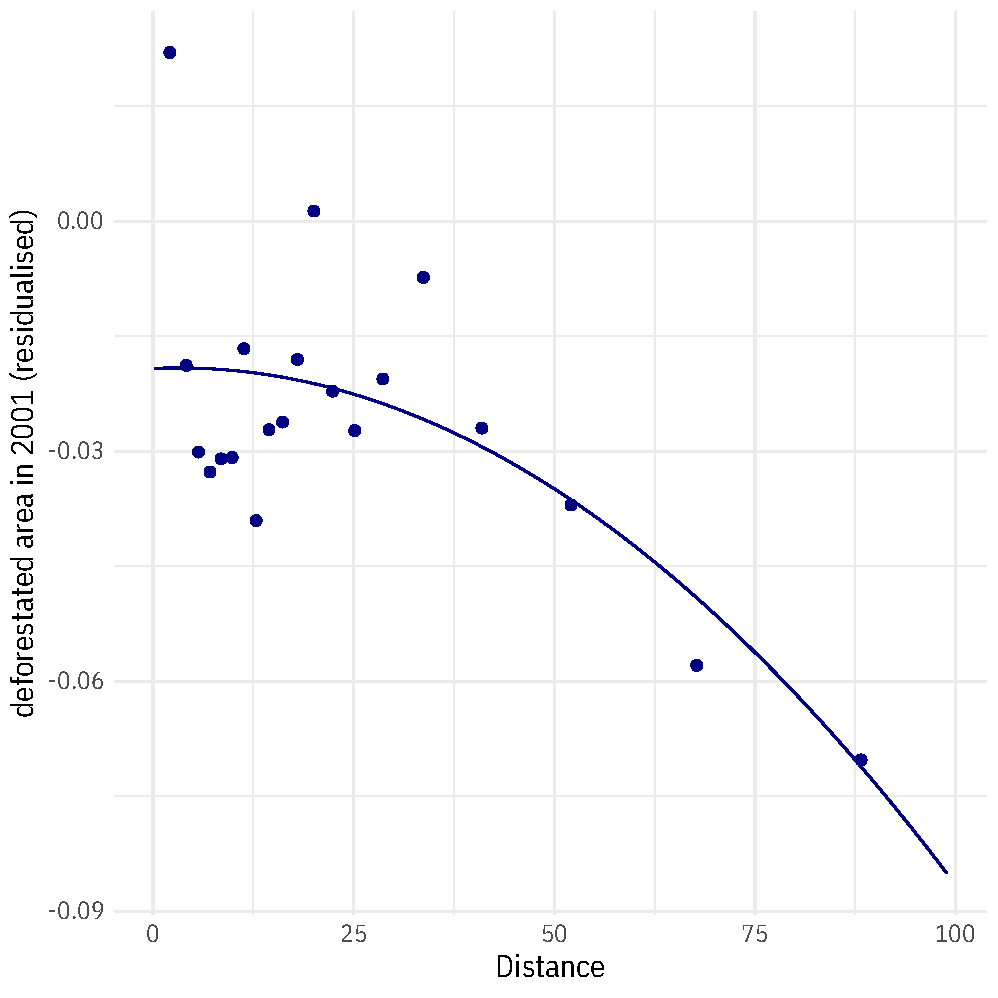
\includegraphics[width=3 in,angle=0]{Output/deforestation_v_mines.pdf}}
\end{minipage}
\hfill \hfill
\begin{minipage}{0.45 \linewidth}
\caption*{\emph{\textbf{Panel B}: Treatment effects on Annual Deforestation by Distance to Mines}}
\centerline{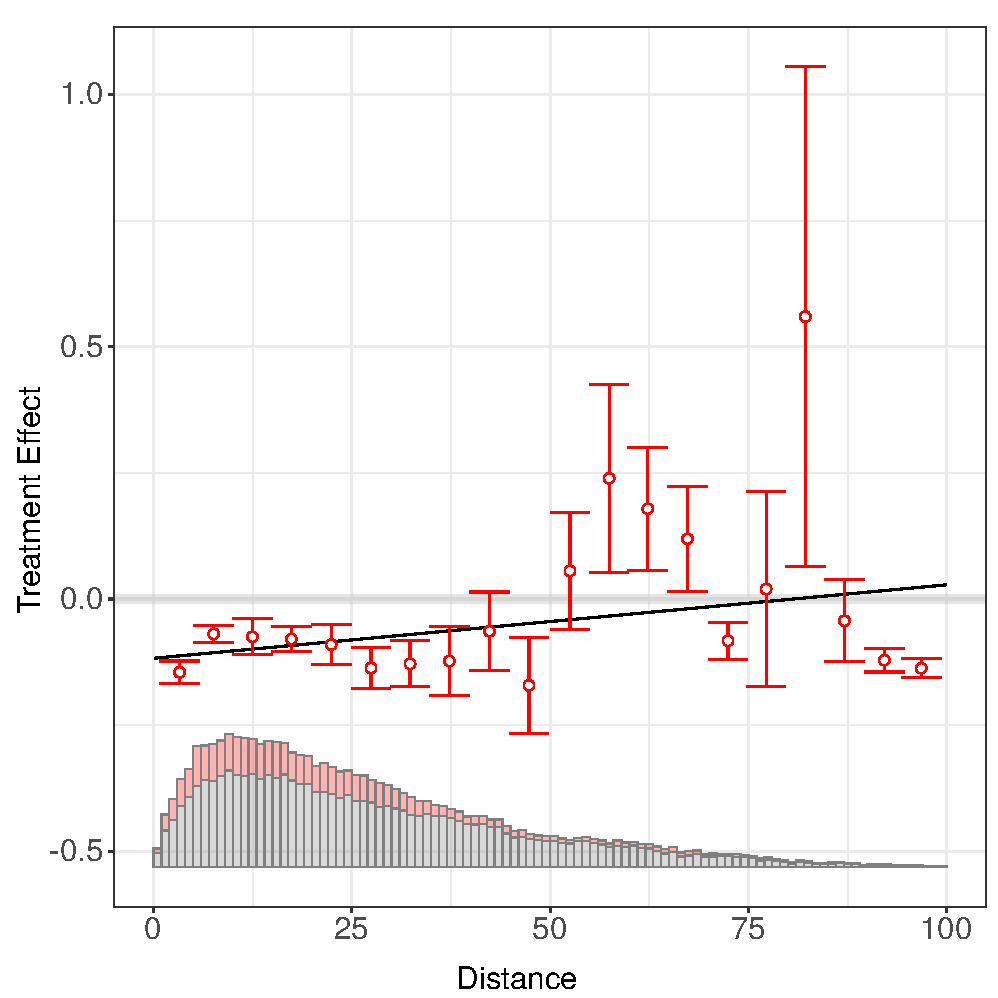
\includegraphics[width=3 in,angle=0]{Output/Interflex_main.pdf}}
\end{minipage}

\emph{Notes for Panel A}: We restrict to these three states because PESA was already implemented in other 5th schedule states by 2001. The figure reports non-parametric binned scatterplot as a function of distance to mines (controlling for pre-2000 forest cover and area - which translates the coefficients below 0 without altering their interpretation). Descriptively, it appears to be the case that the rate of deforestation is higher in areas closer to mines. \\
\emph{Notes for Panel B}:
We report treatment effects from a binned regression that estimates the treatment effect in villages at different values of the moderator (Distance to mines). This approach avoids strong functional forms with-regard to the effect of the moderator, and indeed we find that the interaction effect is nonlinear. Treatment effects are concentrated in villages within 50km from mines.

\end{figure}


\begin{table}[!htbp] \centering \footnotesize
  \caption{Treatment Effects on Annual Deforestation by mine density within 5 km buffer} 
  \label{table:reg_mine_density} 
\begin{tabular}{@{\extracolsep{0pt}}lcc} 
\\[-1.8ex]\hline \\[-1.8ex] 
\\[-1.8ex] & \multicolumn{2}{c}{Annual Deforestation in Hectares} \\ 
\\[-1.8ex] & (1) & (2)\\ 
\hline \\[-1.8ex] 
  Scheduled $\times$ PESA & $-$0.079$^{***}$ & $-$0.080$^{***}$ \\ 
  & (0.008) & (0.009) \\ 
  Scheduled $\times$ PESA $\times$ Number of Mines within 5 km & $-$0.034$^{***}$ &  \\ 
  & (0.009) &  \\ 
  Scheduled $\times$ PESA $\times$ 1-2 Mines within 5 km &  & $-$0.037$^{***}$ \\ 
  &  & (0.013) \\ 
  Scheduled $\times$ PESA $\times$ 3-4 Mines within 5 km &  & $-$0.141$^{***}$ \\ 
  &  & (0.053) \\ 
  Scheduled $\times$ PESA $\times$ 5+ Mines within 5km &  & $-$0.128 \\ 
  &  & (0.133) \\ 
 Village FE & $\checkmark$ & $\checkmark$ \\ 
Year FE & $\checkmark$ & $\checkmark$ \\ 
Dep. Var. Mean & 0.22 & 0.22 \\ 
N. Villages & 52776 & 52776 \\ 
N & 897,192 & 897,192 \\ 
\hline \\[-1.8ex] 
\multicolumn{3}{l}{$^{*}$p $<$ .1; $^{**}$p $<$ .05; $^{***}$p $<$ .01} \\ 
\multicolumn{3}{l}{Cluster-Robust Standard Errors (by village)} \\ 
\end{tabular} 
\end{table} 



\subsection{Unpacking Representation: The Case of Jharkhand\label{jharkhand}}

Improved representation in our context comprises two elements: local government and mandated representation for ST. While we have made the case for the importance of both, the case of Jharkhand allows some insight of the relative impact of quotas on deforestation. Due to legal battles regarding the independence of the state of Jharkhand  -- before 2000, Jharkhand was a part of Bihar -- Jharkhand held its first local elections for \emph{both} Scheduled and non-Scheduled Areas together in 2010. For this reason, Jharkhand's first post-PESA election in 2010 introduced local elections effectively to the entire state, and ST quotas-only in Scheduled Areas. 

The case of Jharkhand is therefore a good candidate to decompose the treatment effects we observe because local government, via local elections, arrives in both Scheduled and non-Scheduled Areas at the same time. Consequently, any treatment effects we observe in this state are more likely attributable to mandated representation for ST via quotas instead of the existence of local government. On the other hand, if we do not observe any treatment effects, then quotas are less likely to be the key element of improved representation for ST. Consistent with the first story, we find strong effects of the treatment in Jharkhand as shown in Appendix Table ~\ref{table:regres_by_state}. This suggests that mandated representation was a key element in addressing the historical absence of political voice for ST in rural India.

%, alongside Chhattisgarh and Uttrakhand
% Jharkhand, because of its separation as an independent state from Bihar in 2000, 

% Jhkarhand first held local elections in both Scheduled and non-Scheduled Areas at the same time, in 2010. This was due to its separation from Bihar in 2000 as an Independent state. 

% did not hold local elections anywhere in the state until 2010, after PESA was introduced. 





% We interpret this difference as suggesting in Jharkhand, where both Scheduled and non-Scheduled Areas lacked a history of local elections, the quota made a dramatic impact in 2010. 









%  ######   #######  ##    ##  ######
% ##    ## ##     ## ###   ## ##    ##
% ##       ##     ## ####  ## ##
% ##       ##     ## ## ## ## ##
% ##       ##     ## ##  #### ##
% ##    ## ##     ## ##   ### ##    ##
%  ######   #######  ##    ##  ######


\section{Discussion: Conservation and Development} % (fold)
\label{sec:conclusion}


%\subsection{Conservation and Development}
%\subsection{Debates around Conservation and Development}

%Scholars have long debated whether empowering local government institutions exacerbates or attenuates the overuse of common pool resources. one hand, central control allows the policy-maker to account for externalities in their resource-use decisions \parencite{hardin1968tragedy}. On the other, scholars have suggested that local control can, in fact, be an effective tool to ward off overuse \parencite{ostrom1990governing}. 

The British Colonial government justified exclusive-use policies over India's forest lands with the spectre of rural villagers spoiling those very lands, policies reinforced in turn by the nascent Indian state. As this narrative of extraction faded in contemporary India, a new debate arose pitting those who favor large-scale `development' against others favoring `environmentalism.' However, the presentation of development and conservation as trade-offs raises a key question: to whose development and welfare are critics and analysts referring? 

Critics characterize conservation advocates as elites who are unaware of the marginalization and impoverishment of rural communities outside of their urban circles. \textcite[57]{guha1992prehistory} writes that ``... the Indian environmental debate is an argument in the cities about what is happening in the countryside.'' Even prominent politicians shrug off environmentalists as aiming to only save ``tigers and trees,'' without any regard to local development \parencite[235]{baviskar1995belly}. For these elites, `development' means large-scale industrial projects -- corporate endeavors that clear forests and displace local communities.


%Given the out-sized effects of these historical policies on India's Scheduled Tribes, who have depended upon forests for economic well-being and livelihoods, the boost in representation we evaluate here, provides a robust test as to whether giving greater formal political control to marginalized communities leads to greater extraction or protection of forest resources -- an area of great debate even within India \parencite[Chapter 5]{kashwan2017democracy}. 

%% Not sure this next part is right ... activists say 'development' is evil because they mean industry

%\todo{discuss development as industrialization vs development as welfare}


Other voices, focused on the lives and livelihoods of the most marginalized rural communities, are focused more on distributional concerns. These are usually local interests who are closer to or from affected communities. For instance, when one of the authors lived and completed fieldwork at a research institute in Ranchi, Jharkhand in the Summer of 2014, local economists and activists, separately, stressed to him a tension between the aims of local economic growth with the rights and interests of local, marginalized communities. If `development' is understood as focused on improving the welfare of local, impoverished communities, then the Scheduled Tribes are as \textcite[239]{baviskar1995belly} describes, ``environmentalists by default'' as ``their present resource use can be called sustainable... if we compare it with the vastly more destructive practices of the state and the market.'' 


%At the very least, against a counterfactual of bureaucratic control, the use of local resources by these communities is very likely to be less exploitative.  makes this point by calling communities like Scheduled Tribes ``environmentalists by default''  because ``their present resource use can be called sustainable only if we compare it with the vastly more destructive practices of the state and the market'' (p. 239). 

%The first relates to the lives of local communities, particularly those like the Scheduled Tribes in India, are linked closely with ecological concerns. These are precisely the communities are most likely to use forest resources in a sustainable manner. 


%To place the results in the development-conservation debate,

%\subsection{Evidence on Conservation and Development}

Our evidence supports the latter view. The evidence we present on conservation here can be read in conjunction with other work that evaluates the impact of the same institution on development outcomes. \textcite{gulzar2019} show that increased political representation for Scheduled Tribes also improved their economic well-being. They examine impacts on the performance of the world's largest employment program, the National Rural Employment Guarantee Scheme (NREGS), India's flagship social protection program, which aims to guarantee a hundred days of minimum wage labor, to every Indian citizen, each year. 
They find that mandated representation for ST significantly boosts how much work ST receive under this program without compromising overall implementation of NREGS. Finally, they also document economic benefits beyond NREGS through improvements in local public goods and road connectivity.

Taken together, our findings and the results in \textcite{gulzar2019}, suggest that development and conservation need not be substitutes. To be clear, these two sets of results do not offer a full accounting of welfare, the calculation of which requires more granular data, a consistent research design, and a model for counterfactual welfare calculations. Rather, in placing our results in conversation with related evidence in \textcite{gulzar2019}, we advocate for scholars and policymakers to pay closer attention to what we describe as `umbrella institutions': institutions, such as political representation, which hold promise in meeting multiple objectives, such as development and conservation, in tandem. This contrasts with the more common approach of focusing on the impact of institutions specifically designed to promote conservation (such as, for instance, community driven forestry), and separately, examining how development promoting institutions affect development.


%...contrary to how debates between on conservation and development are typically set up, we find that political representation is an institution that can deliver improvements in conservation and development in tandem.




% More broadly, examining the impacts of political quotas, an important tool in the design of political institutions across the world, is also significant because it represents a mechanism by which potential policy trade-offs can be resolved through democratic means.

%In summary, we find that a law introducing local government quotas for disadvantaged groups substantially reduced the rate of deforestation in Indian villages. We provide suggestive evidence in favour of an electoral control mechanism -- that PESA reservations resulted in ST politicians gaining greater electoral control and in turn reducing resource extraction. We hypothesise that the election of ST leaders to local councils improved enforcement, thereby reflecting the strong preservation norms among the scheduled tribes in village policy. Endowing political and bureaucratic power at administrative units congruent with networks at which informal norms of preservation exist may improve the effectiveness of environmental preservation -- by lowering enforcement costs -- and adding administrative frictions that render illegal overuse more costly.

%We find evidence that local governments can be effective in promoting environmental protection, especially when key stakeholders, such as ST in India, are included pro-actively. This finding runs counter to the argument that administrative unit proliferation and decentralisation create incentives for over-extraction by exacerbating collective action problems. By contrast, we find suggestive evidence that collective action problems were overcome by informal institutions, within identity-based communities, that enforced norms of sustainable resource use.



%A second contribution is to examine how formal political representation optimizes policy on multiple dimensions simultaneously. This contrasts with policies and institutions that focus exclusively on conservation. Around the world politicians in rural local governments serve under a broad mandate that includes many considerations of local development. These development imperatives include bettering the livelihoods of rural populations, who are frequently poor and marginalized, in addition to  considerations of how best to use and protect local natural resources. The first role relates to local governments' decisions on implementing large-scale social protection programs as well as infrastructure in their communities. The second role relates to a host of decisions that have a direct impact on deforestation, including negotiating with higher level government officials and corporate interests. These negotiations may facilitate or block new mining projects, affect patterns of logging, and access by rural populations to forest products. Institutions that are able to tackle both development and conservation in tandem may be particularly impactful, and thus attractive to policymakers.

%To what extent does increasing representation, for instance by means of mandated representation via quotas, improve targeted communities interests beyond renewable resources? Scholars have shown quotas to be an effective tool in representing the interests of marginalized populations for public goods and the provision of government programs more broadly.\footnote{See for instance \textcite{chattopadhyayWomenPolicyMakers2004,jensenius2017social}, [citation omitted]} But a critical question remains -- do increases in local development come at the cost of conservation? On one hand, as critics of empowering local communities vis-a-vis forests argue, these positive development impacts may come at the cost of over-extracting forest resources. On the other hand, as the lives of these communities is intimately linked with forests, there are good reasons to believe that their use of forest resources will be less extractive than under central control. We examine these competing claims empirically and return to the implied trade-off between development and conservation in Section \ref{sec:conclusion}.

\section{Conclusion}

% Overall, this paper evaluates the impact of representation on forest conservation. 

This paper shows that local representation matters for natural resource conservation. We find that the introduction of local government elections and quotas for Scheduled Tribes substantially reduces the rate of deforestation across Indian villages. We probe and provide evidence for an important mechanism that popular accounts of conflict around deforestation have referenced -- mining interests. We find that the reduction in deforestation is largest in areas closest to mines, suggesting that with improved representation politicians are able to undermine the influence of corporate mining interests.


% section conclusion (end)

Examining the impact of political representation carries important implications beyond the case of India. More than 100 countries have adopted political quotas to empower marginalized communities, many of whom are intimately linked with forests. While scholars have examined a variety of institutions that seek to tackle deforestation directly, our focus on electoral representation is an examination of an umbrella policy, one that aims to simultaneously improve the economic welfare of marginalized communities, but also give local populations more control, and hence reduce overuse, of their local resources. Given the prevalence of quotas and the critical importance of resource preservation, political representation as an umbrella approach appears to be well worth further analysis and policy consideration.



%\pagebreak

%%%%%%%%%%%%%%%%%%%%%%%%%%%%%%%%%%%%%%%%%%%%%%%%%%%%%%%%%%%%%

\printbibliography

\newpage
\renewcommand{\thetable}{A\arabic{table}}
\renewcommand{\thefigure}{A\arabic{figure}}
\setcounter{table}{0}
\setcounter{figure}{0}

\appendix

\part{Online Appendix}
\parttoc 
\begin{refsection}


\clearpage
\section{Proofs}\label{sec:tragedy_model}

This section uses notation from and provides proofs to the propositions in section \ref{sec:conceptual_framework}.

\subsection{Proof of proposition \ref{prop:trag_propn}} % (fold)
\label{ssub:proof_to_proposition_prop:trag_propn}


% subsubsection proof_to_proposition_prop:trag_propn (end)
Suppose by contradiction that $X^{fb} >
X^*$. We know that $X^* > 0$ because $p> 0$. Then, $c'(X^{fb}) \geq
c'(X^*) > 0$, which follows from the assumptions on $c(\cdot)$. Then,
the RHS of \ref{eqn:soc_opt} is strictly greater than the RHS of
\ref{eqn:ind_opt}, which is impossible since they are both equal to
zero. Therefore,  $X^* > X^{fb}$

\subsection{Proof of proposition \ref{prop:repr_propn}} % (fold)
\label{ssub:proof_to_proposition_prop:repr_propn}

\textbf{Proof:} Suppose by contradiction that $X^{rep} > X^*$. We know
that $X^{*} > 0$ because $p> 0$, then $(1-\alpha) c_G'(X^{rep}) +
\alpha c_L'(X^{rep}) \geq c_G'(X^*) > 0$, which follows from the
assumption that $c_L'(\cdot) > c_G'(\cdot)$. Then, the right hand side
of \ref{eqn:vil_prob2} is strictly greater than \ref{eqn:vil_prob},
which yields a contradiction since they are both equal to zero. 
Therefore, $X^{rep} < X^{*}$.

% subsubsection proof_to_proposition_prop:repr_propn (end)
% subsection proofs (end)

\newpage

\section{Discussion of Treatment Effect Size\label{treat_size}}
We calculate the implied back of the envelope effect in Section \ref{MainEffects} by multiplying the treatment effect -0.06 with the number of treated villages $15,940$ (of $52,776$ forested villages. Multiplying these produces $-0.06 \text{ Hectares } \times 15,940 = 1434.6$ hectares. Very roughly assuming that there are 1000 trees per hectare means that treatments prevented an average loss of 1.4 million trees annually compared to control areas.


\newpage
\section{Additional Tables}

\footnotesize

\subsection{Summary Statistics} % (fold)
\label{ssub:summary_statistics}

\begin{centering}
\begin{table}[!htbp] \centering
  \caption{Summary Statistics for main analysis sample (forested; ex-ante forest cover over 2\%)}
    \label{table:sumstats0}
    \scalebox{0.9}{
    
\begin{tabular}{@{\extracolsep{5pt}}lccccccc} 
\\[-1.8ex]\hline 
\hline \\[-1.8ex] 
Statistic & \multicolumn{1}{c}{N} & \multicolumn{1}{c}{Mean} & \multicolumn{1}{c}{St. Dev.} & \multicolumn{1}{c}{Min} & \multicolumn{1}{c}{Pctl(25)} & \multicolumn{1}{c}{Pctl(75)} & \multicolumn{1}{c}{Max} \\ 
\hline \\[-1.8ex] 
\# households & 52,270 & 169.100 & 972.500 & 1 & 40 & 172 & 187,059 \\ 
Population & 52,270 & 742.700 & 4,159.000 & 10 & 178 & 772 & 809,378 \\ 
Scheduled & 52,270 & 0.303 & 0.459 & 0 & 0 & 1 & 1 \\ 
2000 Forest Index (Max) & 52,270 & 69.360 & 19.190 & 9 & 54 & 85 & 100 \\ 
200 Forest Index (Mean) & 52,270 & 16.470 & 15.630 & 2.000 & 4.452 & 24.360 & 89.100 \\ 
Number of Cells & 52,270 & 6,483.000 & 11,673.000 & 10 & 1,531 & 7,750 & 1,097,168 \\ 
ST Share & 52,270 & 0.508 & 0.413 & 0.000 & 0.005 & 0.945 & 1.000 \\ 
SC Share & 52,270 & 0.103 & 0.179 & 0.000 & 0.000 & 0.134 & 1.000 \\ 
\hline \\[-1.8ex] 
\end{tabular} 

    }
\end{table}
\end{centering}


\begin{centering}
\begin{table}[!htbp] \centering
  \caption{Summary Statistics for entire sample}
  \label{table:sumstats1}
  \scalebox{0.9}{
    
\begin{tabular}{@{\extracolsep{5pt}}lccccccc} 
\\[-1.8ex]\hline 
\hline \\[-1.8ex] 
Statistic & \multicolumn{1}{c}{N} & \multicolumn{1}{c}{Mean} & \multicolumn{1}{c}{St. Dev.} & \multicolumn{1}{c}{Min} & \multicolumn{1}{c}{Pctl(25)} & \multicolumn{1}{c}{Pctl(75)} & \multicolumn{1}{c}{Max} \\ 
\hline \\[-1.8ex] 
\# households & 285,182 & 333.700 & 1,833.000 & 1 & 80 & 316 & 248,162 \\ 
Population & 285,182 & 1,561.000 & 8,455.000 & 10 & 374 & 1,501 & 977,771 \\ 
Scheduled & 285,182 & 0.187 & 0.390 & 0 & 0 & 0 & 1 \\ 
2000 Forest Index (Max) & 285,182 & 28.300 & 27.570 & 0 & 6 & 45 & 100 \\ 
200 Forest Index (Mean) & 285,182 & 3.167 & 9.197 & 0.000 & 0.007 & 0.684 & 89.100 \\ 
Number of Cells & 285,182 & 7,728.000 & 12,621.000 & 5 & 2,271 & 9,156.0 & 1,236,411 \\ 
ST Share & 285,182 & 0.282 & 0.364 & 0.000 & 0.000 & 0.549 & 1.000 \\ 
SC Share & 285,182 & 0.143 & 0.178 & 0 & 0.002 & 0.2 & 1 \\ 
\hline \\[-1.8ex] 
\end{tabular} 

    }
\end{table}
\end{centering}


% subsubsection summary_statistics (end)

\pagebreak

\normalsize

\subsection{Auxiliary Regression Estimates \label{sub:auxreg}}

% \pagebreak
\begin{table}[htbp!] \centering
  \label{table:vcf_estimates}
  \caption{Analysis using alternate measure of forest cover, the Vegetation Continuous Fields (VCF) measure. This measure is typically far more aggregated and has lower resolution. VCF merges from \textcite{almn2020}.}
{
\def\sym#1{\ifmmode^{#1}\else\(^{#1}\)\fi}
\begin{tabular}{l*{6}{c}}
\hline\hline
                    &\multicolumn{1}{c}{(1)}&\multicolumn{1}{c}{(2)}&\multicolumn{1}{c}{(3)}&\multicolumn{1}{c}{(4)}&\multicolumn{1}{c}{(5)}&\multicolumn{1}{c}{(6)}\\
                    &\multicolumn{1}{c}{Full Sample}&\multicolumn{1}{c}{Full Sample}&\multicolumn{1}{c}{Full Sample}&\multicolumn{1}{c}{Forested}&\multicolumn{1}{c}{Forested}&\multicolumn{1}{c}{Forested}\\
\hline
Scheduled X PESA &     -0.0520\sym{***}&     -0.0347\sym{***}&     -0.0144\sym{***}&     -0.0690\sym{***}&     -0.0480\sym{***}&     -0.0186\sym{***}\\
                    &  (0.000959)         &   (0.00158)         &   (0.00117)         &   (0.00122)         &   (0.00198)         &   (0.00150)         \\
\hline
N X T               &     4457760         &     4457760         &     4457760         &     2674305         &     2674305         &     2674305         \\
Villages (N)        &      297182         &      297182         &      297182         &      178285         &      178285         &      178285         \\
Dep Var Mean        &        1.88         &        1.88         &        1.88         &        2.22         &        2.22         &        2.22         \\
Village FE          &         yes         &         yes         &         yes         &         yes         &         yes         &         yes         \\
Year FE             &         yes         &         yes         &         yes         &         yes         &         yes         &         yes         \\
Village Time Trends &          no         &         yes         &          no         &          no         &         yes         &          no         \\
State-Year FE       &          no         &          no         &         yes         &          no         &          no         &         yes         \\
\hline\hline
\multicolumn{7}{l}{\footnotesize Standard errors in parentheses}\\
\multicolumn{7}{l}{\footnotesize Cluster-Robust SEs by village}\\
\multicolumn{7}{l}{\footnotesize \sym{*} \(p<0.10\), \sym{**} \(p<0.05\), \sym{***} \(p<0.01\)}\\
\end{tabular}
}

\end{table}

% \begin{centering}
% \begin{table}[!htbp] \centering
%   \caption{Village Level Regressions clustered at Block level}
%   \label{table:regres2}
%   \input{Output/fe_estimates_ha_block}
%     % \include{Output/fe_estimates_stata}
% \end{table}
% \end{centering}

\begin{table}[!htbp] \centering 
  \caption{Village level regressions clustered at block level} 
  \label{table:regres2} 
\begin{tabular}{@{\extracolsep{0pt}}lcccc} 
\\[-1.8ex]\hline \\[-1.8ex] 
\\[-1.8ex] & \multicolumn{4}{c}{Annual Deforestation in Hectares} \\ 
\\[-1.8ex] & (1) & (2) & (3) & (4)\\ 
\hline \\[-1.8ex] 
 Scheduled X PESA & $-$0.088$^{***}$ & $-$0.032 & $-$0.016 & $-$0.067$^{**}$ \\ 
  & (0.020) & (0.027) & (0.019) & (0.032) \\ 
 Village FE & $\checkmark$ & $\checkmark$ & $\checkmark$ & $\checkmark$ \\ 
Year FE & $\checkmark$ & $\checkmark$ &  &  \\ 
Village TT &  & $\checkmark$ &  & $\checkmark$ \\ 
State X Year FE &  &  & $\checkmark$ & $\checkmark$ \\ 
Dep. Var. Mean & 0.22 & 0.22 & 0.22 & 0.22 \\ 
N. Villages & 52776 & 52776 & 52776 & 52776 \\ 
N & 897,192 & 897,192 & 897,192 & 897,192 \\ 
\hline \\[-1.8ex] 
\multicolumn{5}{l}{$^{*}$p $<$ .1; $^{**}$p $<$ .05; $^{***}$p $<$ .01} \\ 
\multicolumn{5}{l}{Cluster-Robust Standard Errors (by block)} \\ 
\end{tabular} 
\end{table} 


% \begin{centering}
% \begin{table}[!htbp] \centering
%   \label{table:fullsamp}
%   \caption{Full sample (including villages with no ex-ante forest cover)}
%   \input{Output/fe_full_estimates_ha_code_2011}
%     % \include{Output/fe_estimates_stata}
% \end{table}
% \end{centering}

Table ~\ref{table:fullsamp} reports regression estimates from including all villages in the 9 states in our sample. The results are difficult to interpret because they include many villages that have no forest cover to begin with.


\begin{table}[!htbp] \centering 
  \caption{Village level regressions for full sample (including villages with no ex-ante forest cover)} 
  \label{table:fullsamp} 
\begin{tabular}{@{\extracolsep{0pt}}lcccc} 
\\[-1.8ex]\hline \\[-1.8ex] 
\\[-1.8ex] & \multicolumn{4}{c}{Annual Deforestation in Hectares} \\ 
\\[-1.8ex] & (1) & (2) & (3) & (4)\\ 
\hline \\[-1.8ex] 
 Scheduled X PESA & $-$0.013$^{***}$ & $-$0.003 & 0.001 & $-$0.010 \\ 
  & (0.005) & (0.008) & (0.005) & (0.009) \\ 
 Village FE & $\checkmark$ & $\checkmark$ & $\checkmark$ & $\checkmark$ \\ 
Year FE & $\checkmark$ & $\checkmark$ &  &  \\ 
Village TT &  & $\checkmark$ &  & $\checkmark$ \\ 
State X Year FE &  &  & $\checkmark$ & $\checkmark$ \\ 
Dep. Var. Mean & 0.05 & 0.05 & 0.05 & 0.05 \\ 
N. Villages & 286910 & 286910 & 286910 & 286910 \\ 
N & 4,877,470 & 4,877,470 & 4,877,470 & 4,877,470 \\ 
\hline \\[-1.8ex] 
\multicolumn{5}{l}{$^{*}$p $<$ .1; $^{**}$p $<$ .05; $^{***}$p $<$ .01} \\ 
\multicolumn{5}{l}{Cluster-Robust Standard Errors (by block)} \\ 
\end{tabular} 
\end{table} 



%\iffalse
\pagebreak
Table ~\ref{table:regres_by_state} reports regression estimates from estimating the preferred specification (equation \ref{styfett}) separately for Jharkhand and the rest of the sample. %on villages from each of the four states that get treated within our analysis period. Estimated effects are zero for Chhatisgarh, and large and negative for the other three states. We suspect that effects are muted in Chhatisgarh due to the long-running Naxalite insurgency in the majority of its districts, where it is plausible that local elected officials had little influence in resource preservation due to violence both before and after the introduction of PESA.



\begin{table}[!htbp] \centering 
  \caption{Main Effects in 4 treated states separated by Jharkahnd and Chhattisgarh, Maharashtra, and Odisha} 
  \label{table:regres_by_state} 
\begin{tabular}{@{\extracolsep{5pt}}lcc} 
\\[-1.8ex]\hline \\[-1.8ex] 
\\[-1.8ex] & \multicolumn{2}{c}{Annual Deforestation in Hectares} \\ 
 & Jharkhand & CH/MH/OR \\ 
\\[-1.8ex] & (1) & (2)\\ 
\hline \\[-1.8ex] 
 Scheduled X PESA & $-$0.082$^{***}$ & $-$0.063$^{***}$ \\ 
  & (0.013) & (0.015) \\ 
 Village FE & $\checkmark$ & $\checkmark$ \\ 
Village TT & $\checkmark$ & $\checkmark$ \\ 
State X Year FE & $\checkmark$ & $\checkmark$ \\ 
Dep. Var. Mean & 0.08 & 0.21 \\ 
N. Villages & 5015 & 26586 \\ 
N & 85,255 & 451,962 \\ 
\hline \\[-1.8ex] 
\multicolumn{3}{l}{$^{*}$p $<$ .1; $^{**}$p $<$ .05; $^{***}$p $<$ .01} \\ 
\multicolumn{3}{l}{Cluster-Robust Standard Errors (by village)} \\ 
\end{tabular} 
\end{table} 

%\fi





% subsection subsection_name (end)

% \paragraph{Varying ex-ante forest cover level}
% \input{Output/varying_cutoff.tex}

\pagebreak
\section{Additional Figures} % (fold)
\subsection{Panel-match diagnostics }

The outcome variable in Figure ~\ref{fig:panelmatchbal} is in standardised units, and therefore less likely to reject balance in
large samples spuriously \parencite{imbens2015causal}. The difference between treatment and
comparison groups is consistently under $0.2$SD, which is the conventional threshold. Matching and visualisation was performed using the \texttt{panelmatch} package accompanying \textcite{Imai2019-kp}.


\begin{figure}[htbp!]
\begin{center}
\begin{minipage}{1 \linewidth}
  \caption{\textbf{Balance in pre-treatment deforestation}}
  \label{fig:panelmatchbal}	
\centerline{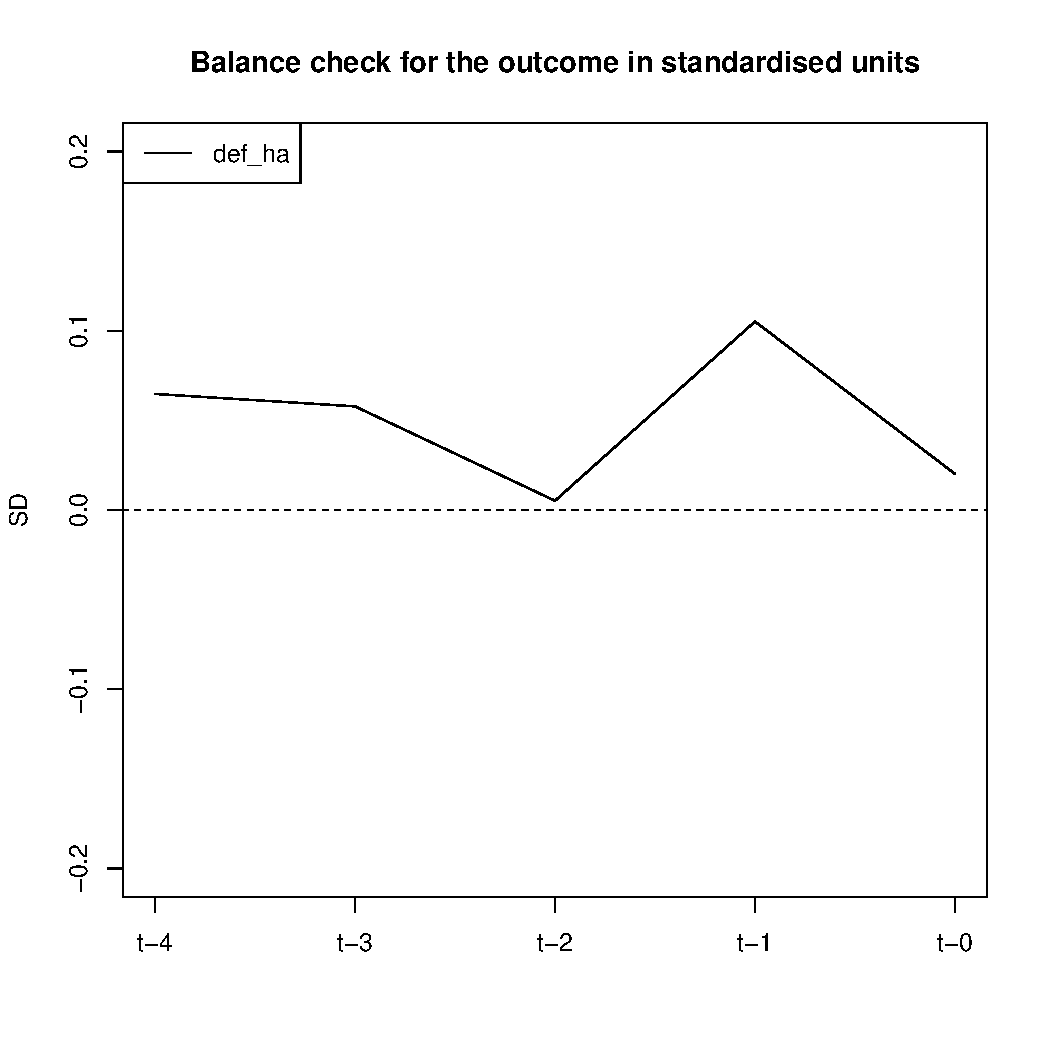
\includegraphics[width=4 in,angle=0]{Output/PanelMatch_bal.pdf}}
\smallskip
\scriptsize
\emph{Notes}: The panelmatch algorithm seeks to match the outcome trajectories of the treatment and control units in the pre-treatment period. The above figure reports the standardised difference between the treatment and control outcomes in the 4 periods before treatment implementation, and in the year of the implementation. We see that consistent with the event study plots ~\ref{fig:autor_plot}, there is some trending in the $t-2$ period, but matching on the trajectory substantially attenuates this imbalance to within 0.1 SD difference.

\end{minipage}
\end{center}
\end{figure}


\pagebreak

\subsection{Mechanisms: Mining}

Here, we report the distribution of mines from the mining atlas (accompanying \textcite{asher2019rent}. We also report 
heterogeneous treatment effects by distance to all available mine types, and by mining density.

\begin{figure}[htbp!]
  \centering
  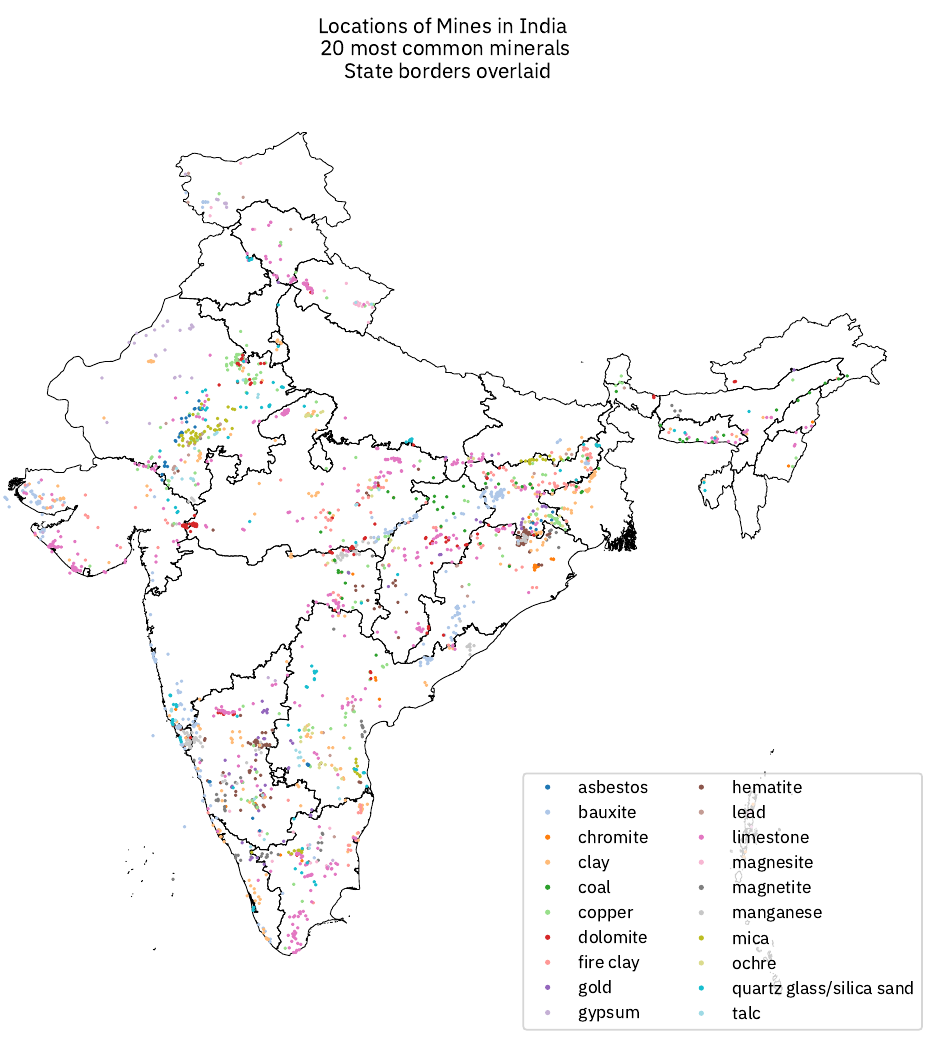
\includegraphics[width=5in,angle=0]{Output/mine_map.png}
  \caption{Location of 20 most common minerals}
  \label{fig:mine_map}
\end{figure}

\pagebreak

\subsubsection{Treatment Effect Heterogeneity}

\begin{figure}[htbp!]
  \centering
  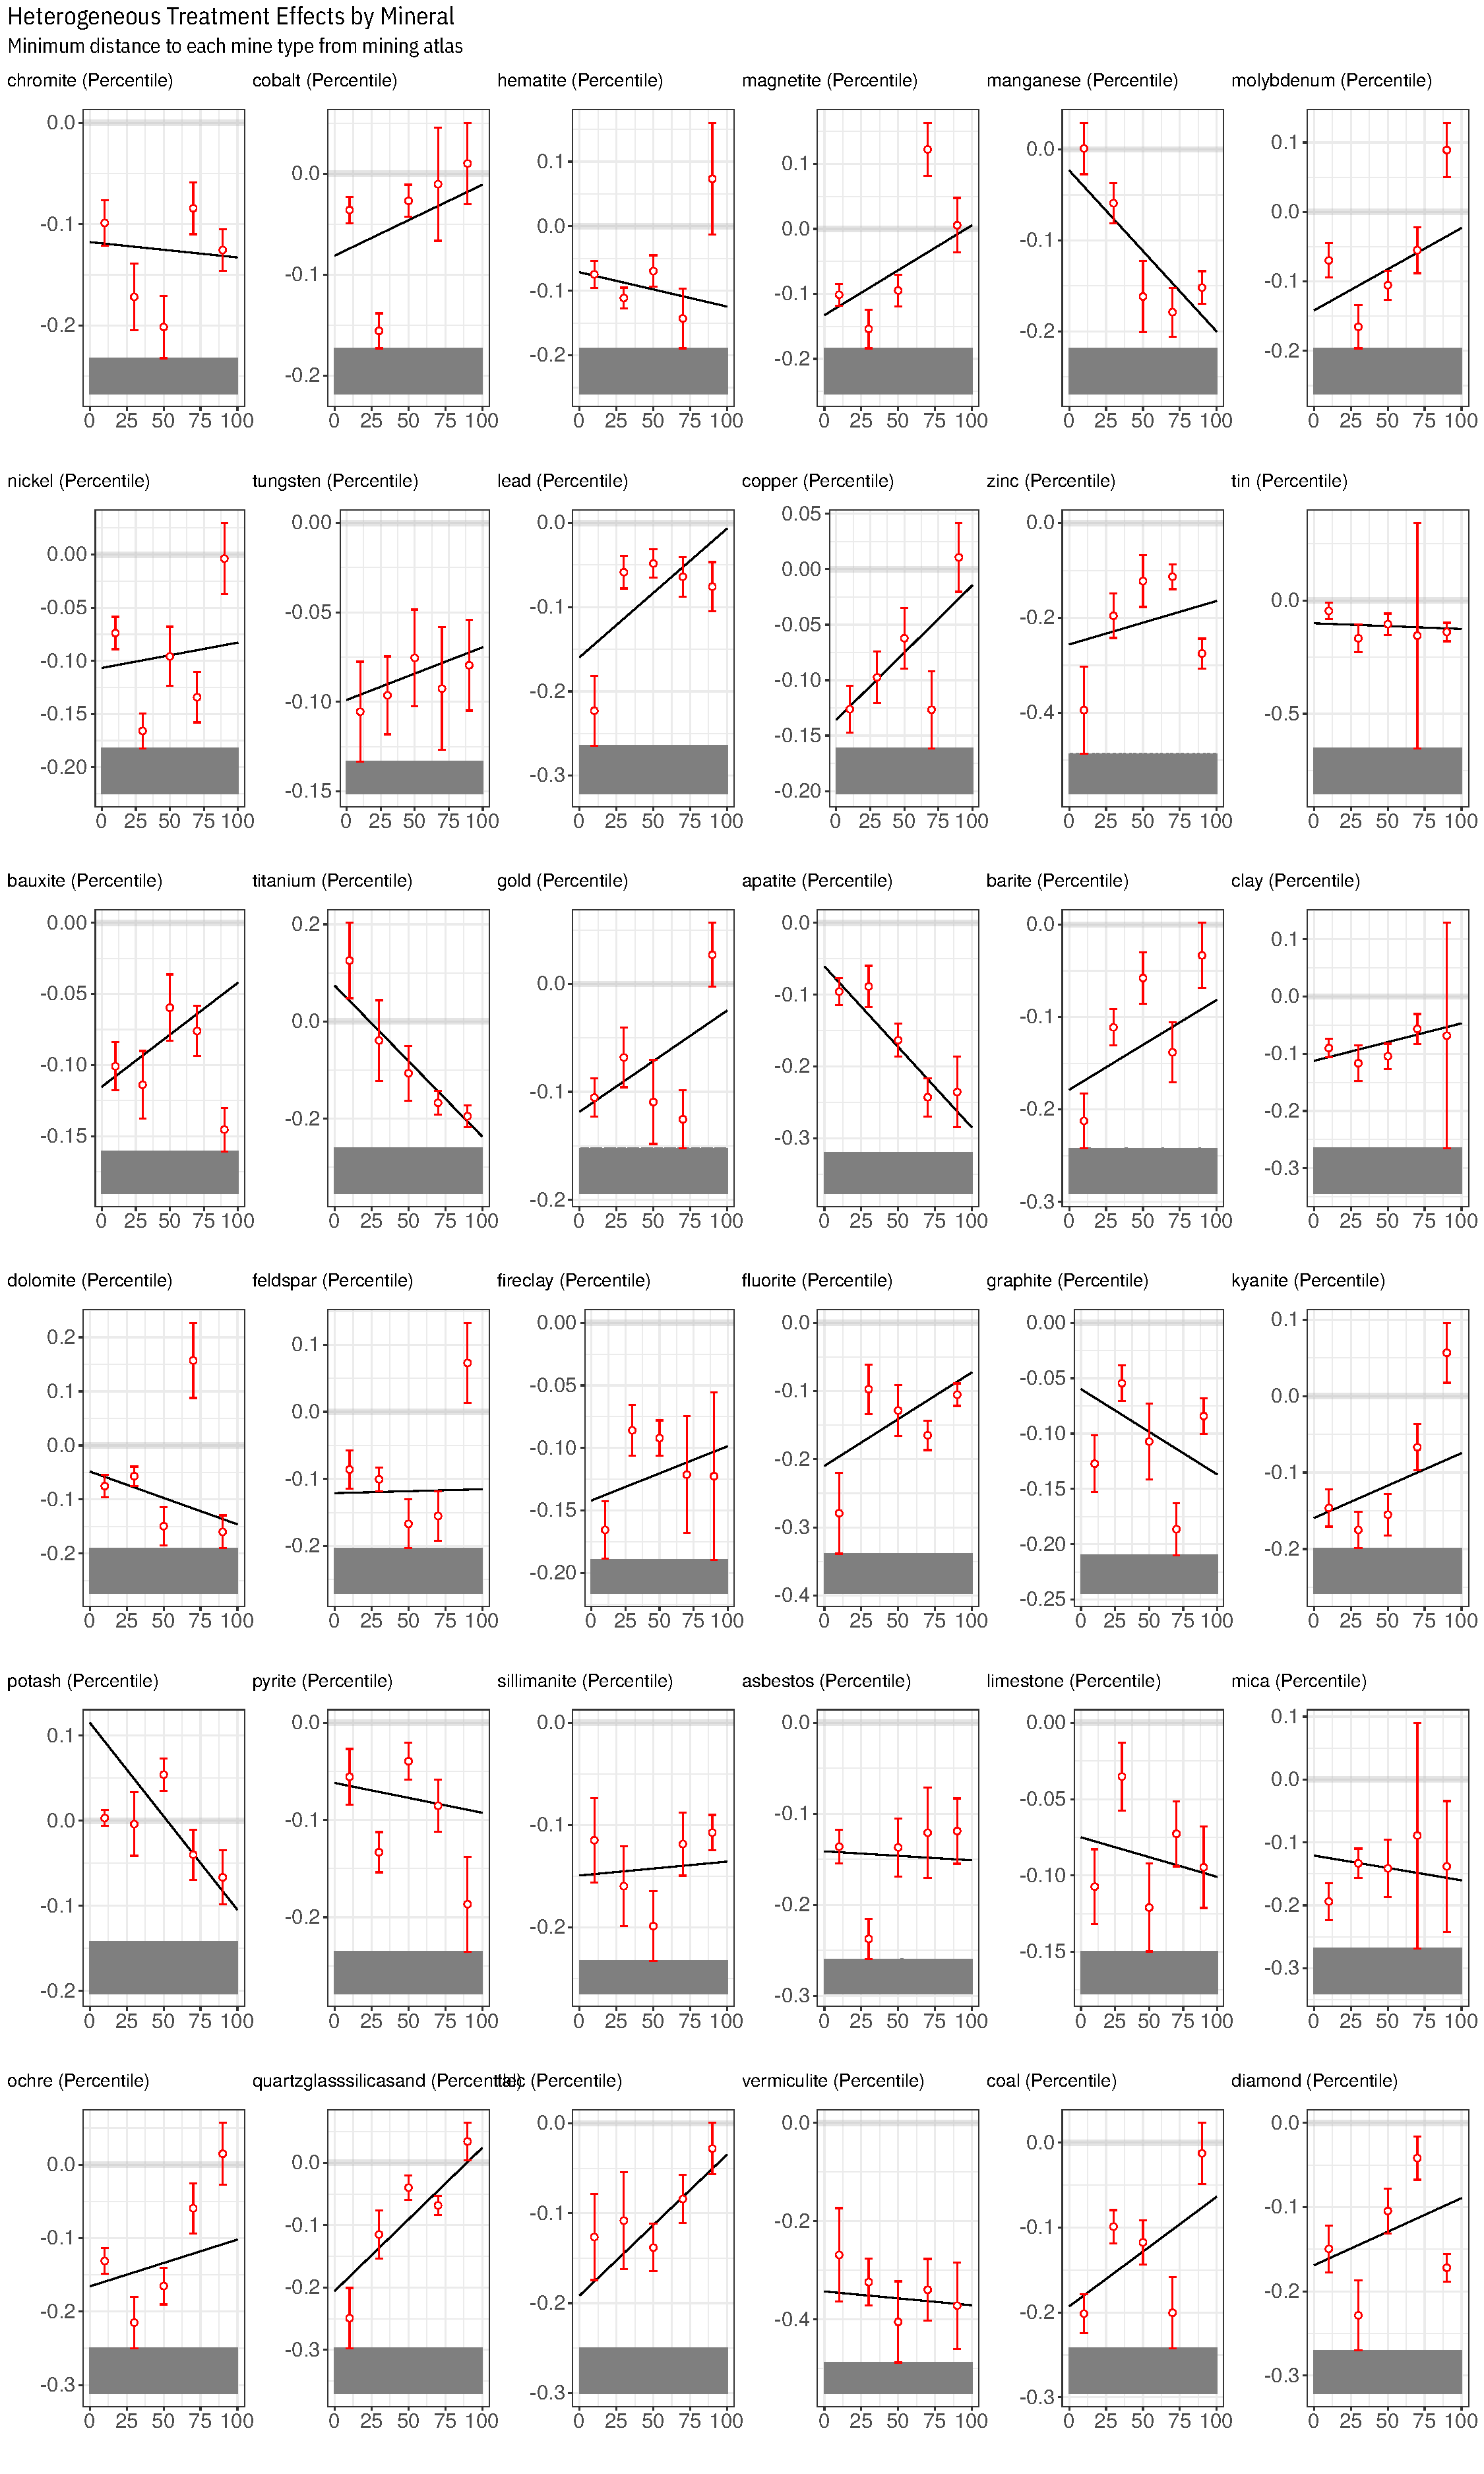
\includegraphics[width = 0.7\textwidth]{Output/mining_het_te.pdf}
  \caption{Interaction effects by mine type}
  \label{fig:mine_het_te}
\end{figure}

%\ref{table:reg_mine_density} reports treatment effects interacted with the number of mines within a 5 km radius of each village (linearly in column 1, and binned in column 2). We find that treatment effects are larger in villages with larger mining intensity in both specifications.



\pagebreak

\subsection{Analysis of Forest Rights Act}


\begin{figure}[htbp!]
  \centering
  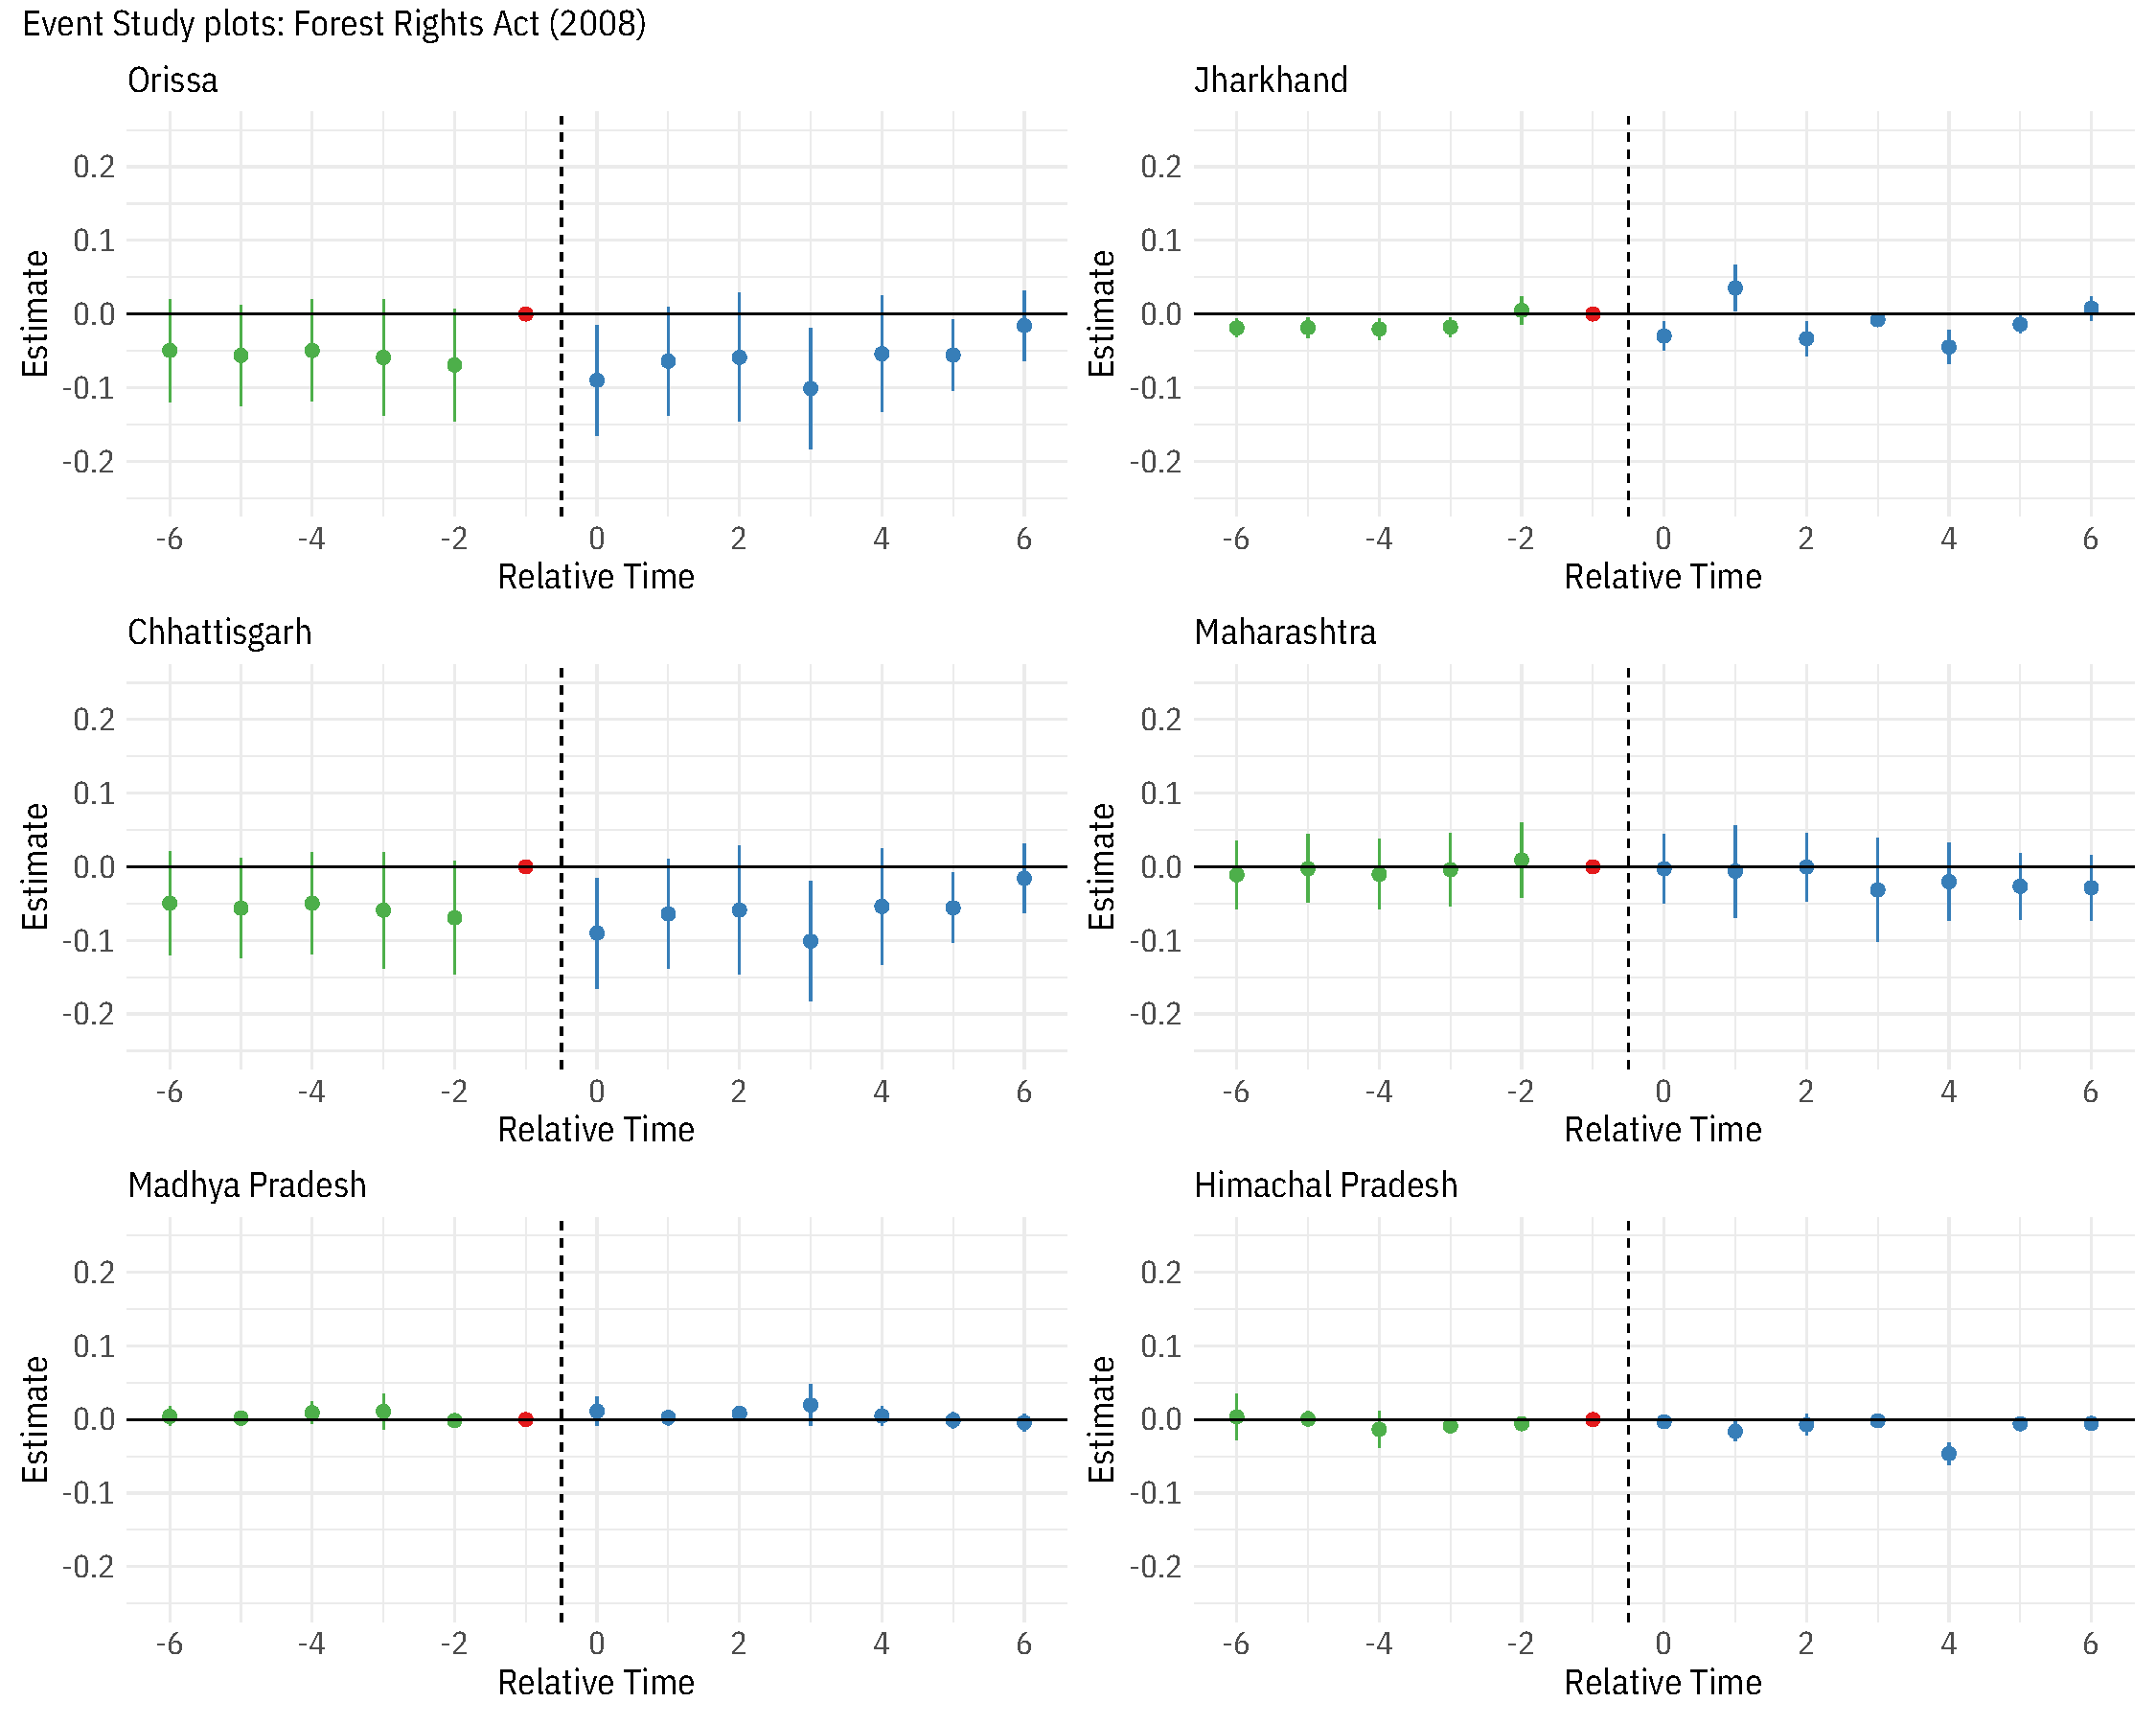
\includegraphics[]{Output/fra_event_studies.pdf}
  \caption{Event Studies by State around the implementation of the Forest Rights Act. We consistently rule out large effects.}
  \label{fig:FRA_evstud}
\end{figure}

\newpage


\section{Software and Data used}
The computation in this paper was performed in R and Python using the following libraries:
\textcite{wickhamGgplot2ElegantGraphics2010}, 
\textcite{wickhamDplyrGrammarData2015}, 
\textcite{gaureLfeLinearGroup2013}, 
\textcite{mckinneyPandasFoundationalPython2011}, 
\textcite{jordahlGeoPandasPythonTools2014}, 
\textcite{waltNumPyArrayStructure2011},
\textcite{hunterMatplotlib2DGraphics2007},
\textcite{hainmueller2019much}, 
\textcite{hlavac2015stargazer},
\textcite{cattaneo2019binscatter},
\textcite{almn2020},
\textcite{dcskkt2015},
\textcite{asher2019rent}, 
\textcite{Hansen2013-vk}

%\clearpage


\printbibliography[heading=subbibliography]
\end{refsection}

%%%%%%%%%%%%%%%%%%%%%%%%%%%%%%%%%%%%%%%%%%%%%%%%%%%%%%%%%%%%%%%
\end{document}


